\documentclass{class}

\usepackage[table]{xcolor}% http://ctan.org/pkg/xcolor
\usetikzlibrary{positioning}
\usepackage{adjustbox}
\usepackage{bbm}
\usepackage{mathrsfs}  
\usepackage{amsmath}% http://ctan.org/pkg/amsmath
\usepackage{tcolorbox}
\setbeamerfont{itemize/enumerate subbody}{size=\normalfont}
\setbeamerfont{itemize/enumerate subsubbody}{size=\normalfont}
\setbeamertemplate{itemize item}{$\bullet$}
\setlength{\leftmargini}{0.25cm}

\title{Self-Selection in Retail Electricity Contracts}
\subtitle{Competition, Regulation, and Welfare Implications}

\author{Léopold Monjoie, Julien Duc}
\institute{Aalto University \and Nantes University}


\apptocmd{\frame}{}{\justifying}{}
\newcommand{\sign}{\text{sign}}
% Conference on Economic Design

\bibliographystyle{apalike}

\begin{document}

\newlength{\tempb}

\frame{\titlepage}

\newcommand{\commentedbox}[2]{%
  \mbox{
    \begin{tabular}[t]{@{}c@{}}
    $\boxed{\displaystyle#1}$\\
    #2
    \end{tabular}%
  }%
}

\newcommand\Wider[2][3em]{%
\makebox[\linewidth][c]{%
  \begin{minipage}{\dimexpr\textwidth+#1\relax}
  \raggedright#2
  \end{minipage}%
  }%
}

\newcommand*\circled[1]{\tikz[baseline=(char.base)]{
            \node[shape=circle,draw,inner sep=2pt] (char) {#1};}}

%%%%%%%%%%%%%%%%%%%%%%%%%%%%%%%%%%%%%%%%%%%%%%%%%%%%%%%%%%%%%%%%%%%%%%%%%%%%%%%%%%%%%%%%%%%%%%%%%%%%%%%%%%%%%%%%%%%%%%%%%%%%%%%%%%%%%%%%%%%%%%%%%%%%%%


\section{Introduction and motivations}

\begin{frame}{Motivations}\label{Motivations}

\begin{mainbox}{Questions}
\begin{itemize}
\vspace{0.15 cm}
    \item  How do heterogeneous consumers self-select into different contracts?
        \vspace{0.15 cm}
    \item How does this sorting interact with retail market equilibrium?
    \vspace{0.15 cm}
\end{itemize}
\end{mainbox}

\vfill

\begin{itemize}    

    \item Fixed Price vs. Dynamic Price contracts. 

    \vfill
   
    \item Uptake of dynamic price contracts increases \boldrblue{allocative efficiency} by reducing the \boldrblue{moral hazard} created by fixed-price contracts. \vfill
    
    \item \textbf{Can welfare loss emerge due to firms reacting to consumers sorting into different contracts?} - \textit{adverse selection}
    \vfill

    \item \textbf{How does it depend on consumer characteristics and market structure}? 
\end{itemize}

       
\end{frame}


%%%%%%%%%%%%%%%%%%%%%%%%%%%%%%%%%%%%%%%%%%%%%%%%%%%%%%%%%%%%%%%%%%%%%%%%%%%%%%%%%%%%%%%%%%%%%%%%%%%%%%%%%%%%%%%%%%%%%%%%%%%%%%%%%%%%%%%%%%%%%%%%%%%%%%

\begin{frame}{Private contracts coexist with regulated options }\label{UptakeContract2}

\begin{figure}
    \centering
    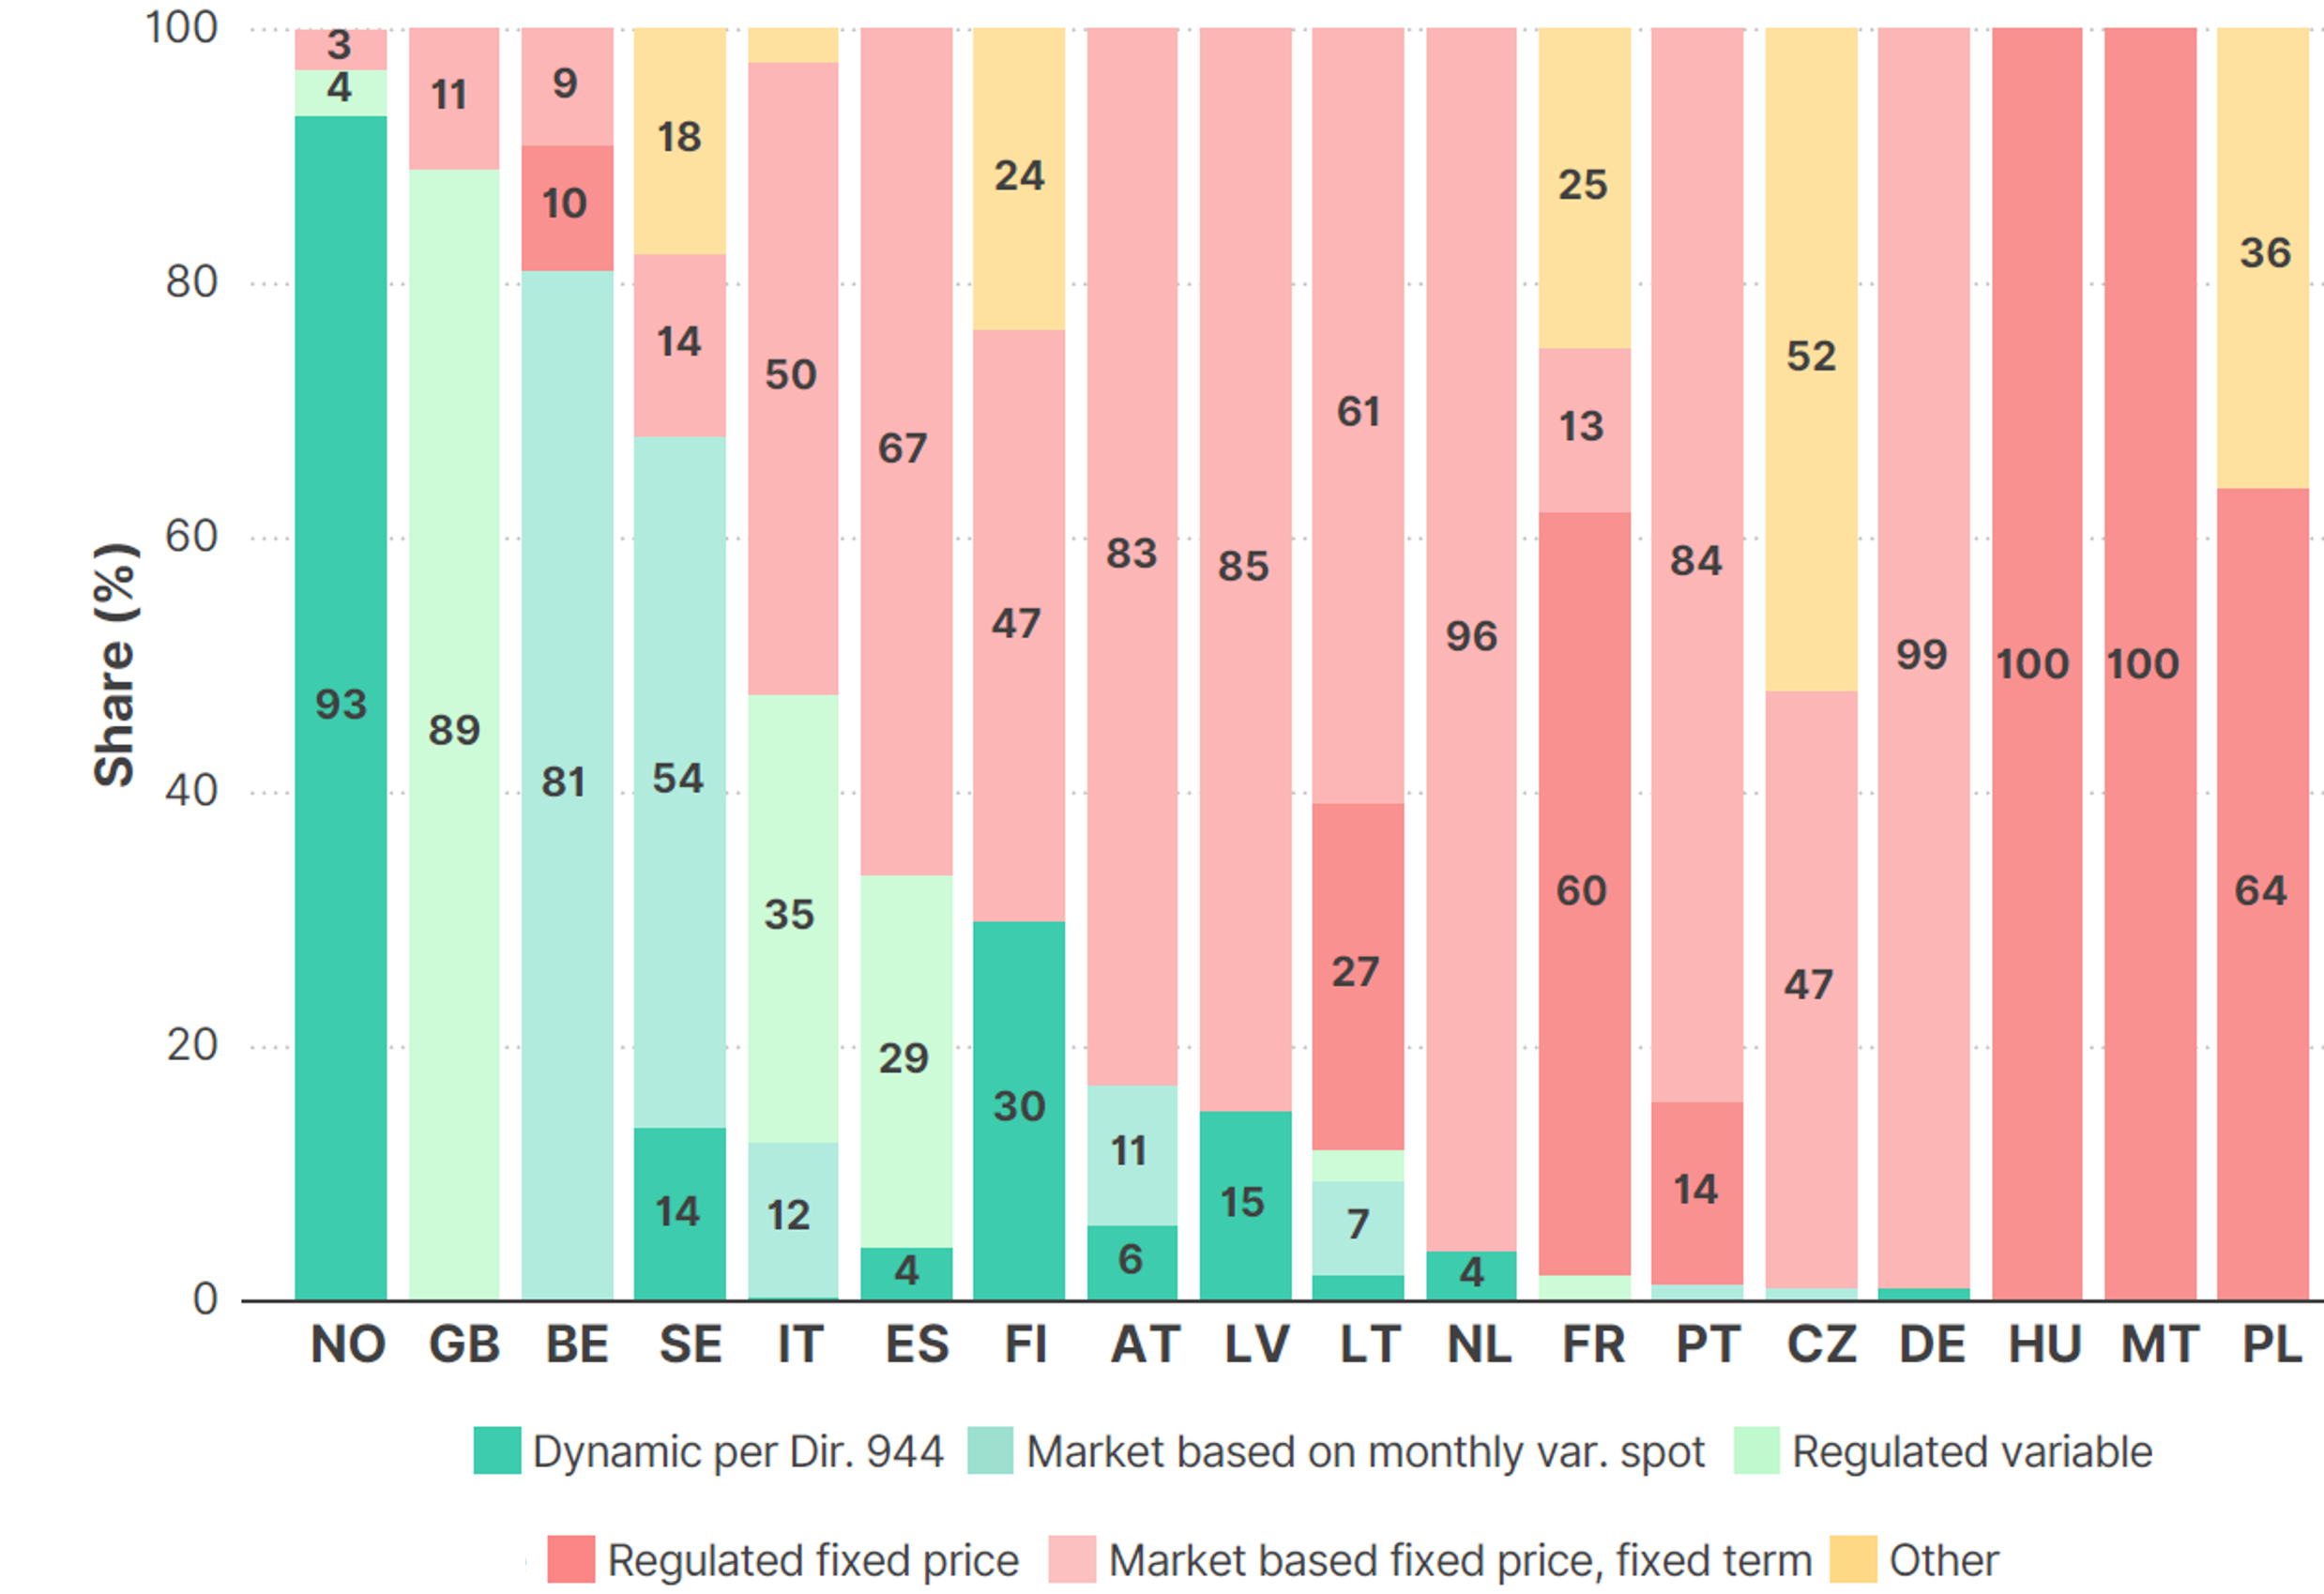
\includegraphics[width=0.8\linewidth]{figure/FP_EU_detail_v2.PNG}
    \caption{Share of household contract uptake in Europe \cite{ACER2024} \hyperlink{options1}{\beamergotobutton{Options}}} 
    \label{fig:FP_EU_detail}
\end{figure}

\end{frame}




%%%%%%%%%%%%%%%%%%%%%%%%%%%%%%%%%%%%%%%%%%%%%%%%%%%%%%%%%%%%%%%%%%%%%%%%%%%%%%%%%%%%%%%%%%%%%%%%%%%%%%%%%%%%%%%%%%%%%%%%%%%%%%%%%%%%%%%%%%%%%%%%%%%%%%



\begin{frame}{First contribution: Demand for contracts with heterogeneous consumers}\label{FirstCont}


\begin{itemize}

\item Provide a \boldrblue{stylized theoretical framework} where a set of consumers have to choose between \boldrblue{a Fixed-Price contract} or \boldrblue{a Dynamic-Price  contract}.

\vfill

\item  Consumers differ in \boldrblue{willingness-to-pay} across consumption period.

\vfill

\begin{itemize}
    \item Extend exogenous share papers. \cite{Borenstein2005b,Leautier2014,Ambec2021,Boom2021}
 
 \vfill
 
 \item Extend single type consumers model. \cite{joskow2006retail,Astier2021,ancel2025tariffs}
    \end{itemize}

\vfill

\end{itemize}

\begin{mainbox}{Partial Equilibrium}
Provide \boldrblue{the demand} for each contract, given a set of prices and the type of consumers who choose each contract.  
\end{mainbox}


\end{frame}



%%%%%%%%%%%%%%%%%%%%%%%%%%%%%%%%%%%%%%%%%%%%%%%%%%%%%%%%%%%%%%%%%%%%%%%%%%%%%%%%%%%%%%%%%%%%%%%%%%%%%%%%%%%%%%%%%%%%%%%%%%%%%%%%%%%%%%%%%%%%%%%%%%%%%%



\begin{frame}{Second contribution: Market equilibrium with consumer choices}\label{SecondCont}


\begin{itemize}

\item We model \boldrblue{retail competition} between firms that offer the two contracts. 

\vfill

\begin{itemize}
    \item Scarce literature \cite{joskow2006retail}, \cite{Borenstein2003} and \cite{ancel2025tariffs}

\vfill

        \item Adverse Selection \cite{1970Akerlof}, price theory \cite{Einav2012}, competition \cite{Azevedo2017}
\vfill

\item Regulation theory \cite{laffont1993theory}, public vs private options \cite{Martimort2020a,Kang2023a}.

\end{itemize}
\end{itemize}


\vfill

\begin{mainbox}{General Equilibrium}
We characterize \boldrblue{the price and welfare equilibrium} in the retail market when consumers can self-select.
\end{mainbox}

\end{frame}



\begin{frame}
\frametitle{Market Structure}
 
\vspace{-2pt}
 
\begin{center}
\scalebox{0.82}{%
\begin{tikzpicture}[node distance=0.45cm]

 \node[draw=notegray!30, fill=white, rounded corners=4pt,
      font=\small\itshape, text=notegray!80,
      inner sep=5pt, minimum width=13cm]
  (banner) at (0,0)
  {Retail Electricity Market};
  
% LEFT: PUBLIC FIRM
\node[firmbox=pubBlue, minimum width=5cm, minimum height=0.95cm,
      below left=0.55cm and 0.3cm of banner.south]
  (pubFirm)
  {\textcolor{pubBlue!15!black}{\textbf{\normalsize Public Firm}}\\[1pt]
   \textcolor{notegray}{\scriptsize regulated monopoly}};
 
\node[contractbox=fixOrange, minimum width=4.2cm,
      below=0.45cm of pubFirm]
  (pubFPC)
  {Fixed-Price Contract};
 
\node[below=0.35cm of pubFPC] (finTitle)
  {\textsc{Financing Mechanisms}};
 
\node[financebox, minimum width=4.2cm, below=0.12cm of finTitle]
  (fin1) {\textbf{(i)} \enspace Self-financing };
 
\node[financebox, minimum width=4.2cm, below=0.1cm of fin1]
  (fin2) {\textbf{(ii)} \enspace Market-wide tax};
 
\node[financebox, minimum width=4.2cm, below=0.1cm of fin2]
  (fin3) {\textbf{(iii)} \enspace Shadow cost of public funds};
 
 
 
% RIGHT: PRIVATE FIRMS
\node[firmbox=privGreen, minimum width=5cm, minimum height=0.95cm,
      below right=0.55cm and 0.3cm of banner.south]
  (privFirm)
  {\textcolor{privGreen!15!black}{\textbf{\normalsize Private Firms}}\\[1pt]
   \textcolor{notegray}{\scriptsize competitive fringe}};
 
\node[contractbox=fixOrange, minimum width=2.1cm, minimum height=1.1cm,
      below left=0.45cm and -2.55cm of privFirm]
  (privFPC)
  {Fixed-Price\\Contract};
 
\node[contractbox=dynPurple, minimum width=2.1cm, minimum height=1.1cm,
      below right=0.45cm and -2.55cm of privFirm]
  (privDPC)
  {Dynamic-Price\\Contract };

\end{tikzpicture}%
}
\end{center}

\vfill

\begin{itemize}
    \item Two market structures: i) private only, ii) public vs. private. 
\end{itemize}
 
\end{frame}


%%%%%%%%%%%%%%%%%%%%%%%%%%%%%%%%%%%%%%%%%%%%%%%%%%%%%%%%%%%%%%%%%%%%%%%%%%%%%%%%%%%%%%%%%%%%%%%%%%%%%%%%%%%%%%%%%%%%%%%%%%%%%%%%%%%%%%%%%%%%%%%%%%%%%%

\begin{frame}{Main takeaways}


\begin{itemize}

\item \boldrblue{A selection market}: cost depends on consumer types and contract choices.


\vfill

\item \boldrblue{Optimal demand for contracts}: Higher willingness to pay during low-price periods $\rightarrow$ dynamic contract. Opposite for the FP contract.

\vfill

\item \boldrblue{Market equilibrium}.

\vfill

\begin{itemize}
    \item \boldrblue{Impossibility result}: FP contracts cannot be sustained at the equilibrium given the selection patterns based on WTP.
    \begin{itemize}
    \vfill
        \item Hold for private firms and a self-financing public firm.
    \end{itemize}
    \vfill

\item \boldrblue{Adverse selection} can be realized with public funds/taxes: \vfill

    \begin{center}
    $W$(\textcolor{blue}{Private} / \textcolor{blue}{Dynamic} + \textcolor{red}{Public} / \textcolor{red}{Fixed-Price})  { \textbf{  < }} $W$( \textcolor{red}{Fixed-Price})
   \end{center}

\vfill

\item Leakage of consumers to the private firms $\rightarrow$ low equilibrium fixed-price.

    \end{itemize}

\end{itemize}


\end{frame}


%%%%%%%%%%%%%%%%%%%%%%%%%%%%%%%%%%%%%%%%%%%%%%%%%%%%%%%%%%%%%%%%%%%%%%%%%%%%%%%%%%%%%%%%%%%%%%%%%%%%%%%%%%%%%%%%%%%%%%%%%%%%%%%%%%%%%%%%%%%%%%%%%%%%%%
%%%%%%%%%%%%%%%%%%%%%%%%%%%%%%%%%%%%%%%%%%%%%%%%%%%%%%%%%%%%%%%%%%%%%%%%%%%%%%%%%%%%%%%%%%%%%%%%%%%%%%%%%%%%%%%%%%%%%%%%%%%%%%%%%%%%%%%%%%%%%%%%%%%%%%
%%%%%%%%%%%%%%%%%%%%%%%%%%%%%%%%%%%%%%%%%%%%%%%%%%%%%%%%%%%%%%%%%%%%%%%%%%%%%%%%%%%%%%%%%%%%%%%%%%%%%%%%%%%%%%%%%%%%%%%%%%%%%%%%%%%%%%%%%%%%%%%%%%%%%%

% \section{The model}

% % \subsection{The environment}

% \begin{frame}{Roadmap}
%   \tableofcontents [sectionstyle=show/shaded,subsectionstyle=show/shaded]
% \end{frame}


%%%%%%%%%%%%%%%%%%%%%%%%%%%%%%%%%%%%%%%%%%%%%%%%%%%%%%%%%%%%%%%%%%%%%%%%%%%%%%%%%%%%%%%%%%%%%%%%%%%%%%%%%%%%%%%%%%%%%%%%%%%%%%%%%%%%%%%%%%%%%%%%%%%%%%


\begin{frame}{Model highlights}


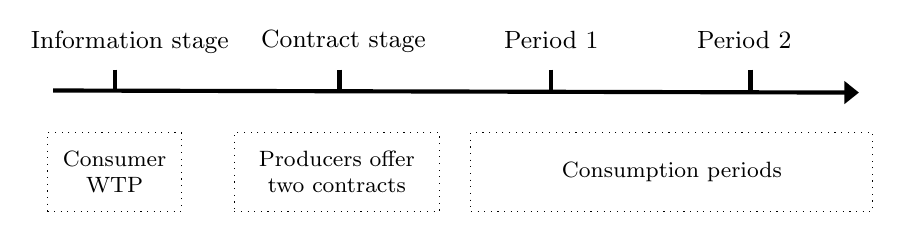
\begin{tikzpicture}[x=0.45pt,y=0.75pt,yscale=-1,xscale=1]

\draw [line width=1.5]    (20,100) -- (663,101) ;
\draw [shift={(667,101)}, rotate = 180.07] [fill={rgb, 255:red, 0; green, 0; blue, 0 }  ][line width=0.08]  [draw opacity=0] (11.61,-5.58) -- (0,0) -- (11.61,5.58) -- cycle    ;
\draw [line width=1.5,color = black]    (70,90) -- (70,100) ;
\draw [line width=1.5,color = black]   (250,90) -- (250,100) ;
\draw [line width=1.5,color = black]   (420,90) -- (420,100)  ;
\draw [line width=1.5,color = black]    (580,90) -- (580,100)   ;

% Text Node
\draw (0,70) node [anchor=north west][inner sep=0.75pt]  [font=\small] [align=center] {Information stage};
\draw (185,70) node [anchor=north west][inner sep=0.75pt]  [font=\small] [align=center] {Contract  stage};
\draw (380,70) node [anchor=north west][inner sep=0.75pt]  [font=\small] [align=center] {Period 1};
\draw (535,70) node [anchor=north west][inner sep=0.75pt]  [font=\small] [align=center] {Period 2};

\draw (15,120) node [draw = black,anchor=north west,minimum height = 1 cm,  text  width = 1.6cm][inner sep=1.5pt,dotted]  [font=\footnotesize] [align=center] {Consumer WTP};
\draw (165,120) node [draw = black,anchor=north west,minimum height = 1 cm,  text  width = 2.5cm][inner sep=1.5pt,dotted]  [font=\footnotesize] [align=center]{ Producers offer \\ two contracts};
\draw (355,120) node [draw = black,anchor=north west,minimum height = 1 cm,  text  width =  5cm,dotted][inner sep=1.5pt]  [font=\footnotesize] [align=center]  { Consumption periods};

\end{tikzpicture}

\begin{itemize}

    \item A unit mass of consumers with a unit demand for electricity for each $t$

\begin{itemize}
    \item WTP: a \boldrblue{two-dimensional} type $\textbf{v}=(v_1,v_2) $
\end{itemize}

    \vfill
        
    \item Perfectly competitive wholesale market w.l.o.g. that $c_1 < c_2$ 

\vfill
        
    \item We assume a set of retailers that purchase at no cost on the wholesale market.

    \vfill

 
    \item If $\textbf{p}^k=(p_1^k,p_2^k)$ is profile unit-price of contract $k$ + fixed part $A^k$, then:  \vfill

    \begin{itemize}
        \item FP contract: $\textbf{p}^{r} =  (p^r,p^r)$ \item Dynamic contract: $\textbf{p}^{s} =  (p_1,p_2)$
    \end{itemize}

\end{itemize}
\end{frame}


%%%%%%%%%%%%%%%%%%%%%%%%%%%%%%%%%%%%%%%%%%%%%%%%%%%%%%%%%%%%%%%%%%%%%%%%%%%%%%%%%%%%%%%%%%%%%%%%%%%%%%%%%%%%%%%%%%%%%%%%%%%%%%%%%%%%%%%%%%%%%%%%%%%%%%



\begin{frame}{Equilibrium Definition - Consumer}


\begin{itemize}

\item The optimal consumer choose a consumption profile $\textbf{x} = (x_1,x_2)$ with $x_t \in\{0,1\}$, given a contract, to maximize its utility:

\vfill

\begin{equation*}
    U(\mathbf{v}, k) = \max_{\mathbf{x} \in \{0,1\}^2} \left\{ \mathbf{x} \cdot (\mathbf{v} - \mathbf{p}^k) - A^k \mathbb{I}_{\{\mathbf{x} \neq \mathbf{0}\}} \right\}
\end{equation*}

\vfill
The \textit{participation set} for contract $k$ is given by:

\begin{equation*} \label{eq:active_set_general}
    \mathcal{S}^k = \left\{ \mathbf{v} \in V : \mathbf{x}^*(\mathbf{v},k) \neq \mathbf{0} \quad \text{and} \quad k \in \arg\max_{j \in \mathcal{K}} U(\mathbf{v}, j) \right\}.
\end{equation*}

\vfill
    
\end{itemize}
    
\end{frame}

%%%%%%%%%%%%%%%%%%%%%%%%%%%%%%%%%%%%%%%%%%%%%%%%%%%%%%%%%%%%%%%%%%%%%%%%%%%%%%%%%%%%%%%%%%%%%%%%%%%%%%%%%%%%%%%%%%%%%%%%%%%%%%%%%%%%%%%%%%%%%%%%%%%%%%



\begin{frame}{Equilibrium Definition}


\begin{itemize}

\item The optimal consumer choose a consumption profile $\textbf{x} = (x_1,x_2)$ with $x_t \in\{0,1\}$, given a contract, to maximize its utility:

\vfill

\begin{equation*}
    U(\mathbf{v}, k) = \max_{\mathbf{x} \in \{0,1\}^2} \left\{ \mathbf{x} \cdot (\mathbf{v} - \mathbf{p}^k) - A^k \mathbb{I}_{\{\mathbf{x} \neq \mathbf{0}\}} \right\}
\end{equation*}

\vfill
The \textit{participation set} for contract $k$ is given by:

\begin{equation*} \label{eq:active_set_general}
    \mathcal{S}^k = \left\{ \mathbf{v} \in V : \mathbf{x}^*(\mathbf{v},k) \neq \mathbf{0} \quad \text{and} \quad k \in \arg\max_{j \in \mathcal{K}} U(\mathbf{v}, j) \right\}.
\end{equation*}

\vfill
    
\item Given a contract $k$, a \textit{private firm} equilibrium is such that:

\vfill

    \begin{equation*}
        \pi^k = \mathbf{q}^k \cdot (\mathbf{p}^k - \mathbf{c}) + \mathbf{A}^k
        \label{eq:private_obj}
    \end{equation*}

\vfill

\item We restrict the \textit{public firm} to offer the fixed-price contract and the equilibrium is such that:

\vfill

    \begin{equation} \label{eq:public_obj}
        \Omega^r = CS^r + (1+\lambda)\pi^r
    \end{equation}

\end{itemize}
    
\end{frame}
%%%%%%%%%%%%%%%%%%%%%%%%%%%%%%%%%%%%%%%%%%%%%%%%%%%%%%%%%%%%%%%%%%%%%%%%%%%%%%%%%%%%%%%%%%%%%%%%%%%%%%%%%%%%%%%%%%%%%%%%%%%%%%%%%%%%%%%%%%%%%%%%%%%%%%


% \begin{frame}{Example with one contract}
% \begin{figure}
%     \centering
%     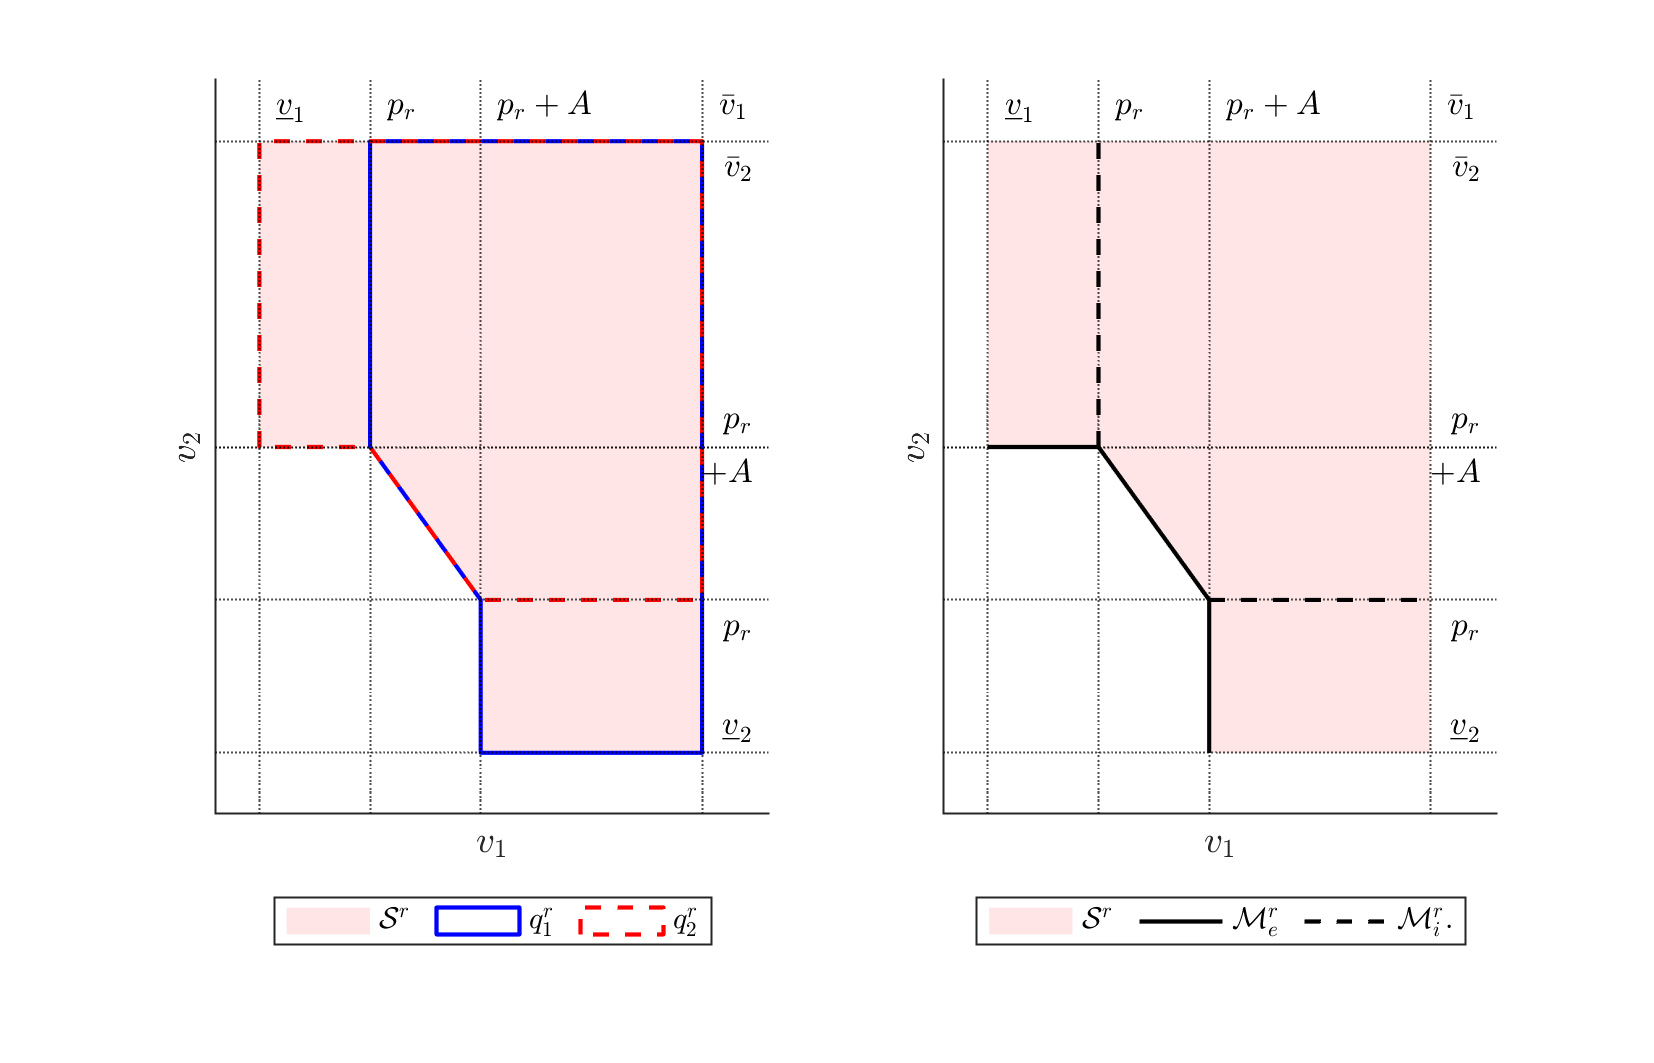
\includegraphics[width=1\linewidth]{figure/intro_zone_A_ppt.png}
%     \caption{Demand for the fixed-price contract, and marginal consumers (\textit{exiters and profile switchers}).}
%     \label{fig:intro_zone_mu}
% \end{figure}


% \end{frame}
% %%%%%%%%%%%%%%%%%%%%%%%%%%%%%%%%%%%%%%%%%%%%%%%%%%%%%%%%%%%%%%%%%%%%%%%%%%%%%%%%%%%%%%%%%%%%%%%%%%%%%%%%%%%%%%%%%%%%%%%%%%%%%%%%%%%%%%%%%%%%%%%%%%%%%%

% \begin{frame}{Single Contract Equilibrium}

% \begin{itemize}

%  \item If private retailers offer the FP contract, then the linear price is the eq. and takes the following form:

% \begin{equation*}
%  p^r^* =  \text{av. total cost}   \quad \text{and} \quad A_r^* =0 
% \end{equation*}

% \vfill

% \item If private retailers offer the RTP contract, then competition implies full cost pass-through to consumers:

% \vfill

% \begin{equation*}
%  \textbf{p}^s^*  = \{p_1^w,p_2^w\}  = \{c_1,c_2\}   \quad \text{and} \quad A_s^* =0 
% \end{equation*}

% \vfill

% \item If the regulated monopoly offers the FP contract, then: 

% \vfill

%         \begin{equation*}
%             p^r^{**} \quad = \quad \text{av.marg.cost} \quad + \quad \text{ramsey A}  \quad- \quad \underbrace{\bigg.A^{**}_r \frac{\delta_A\mu_r}{\delta_A q^r} \bigg.}_{\text{switchers wedge}}
%         \end{equation*}



% \end{itemize}

% \end{frame}

%%%%%%%%%%%%%%%%%%%%%%%%%%%%%%%%%%%%%%%%%%%%%%%%%%%%%%%%%%%%%%%%%%%%%%%%%%%%%%%%%%%%%%%%%%%%%%%%%%%%%%%%%%%%%%%%%%%%%%%%%%%%%%%%%%%%%%%%%%%%%%%%%%%%%%

% \begin{frame}{Adverse Selection in Single Contract Equilibrium}

% \begin{itemize}

% \item We derive sufficient and necessary conditions for the private and public equilibrium to exhibit adverse (or advantageous) selection.  \vfill

% \item  Private equilibrium (sufficient conditions):   \vfill

% \begin{equation*}
%  \frac{\# \text{marginal cons. in 1}}{\# \text{ cons. in 1}} > \frac{\# \text{marginal cons. in 2}}{\# \text{ cons. in 2}}   
% \end{equation*}

% \vfill

% \item  Public equilibrium (necessary conditions):   \vfill

% \begin{equation*}
%  \frac{\# \text{profile switchers in 1}}{\# \text{ cons. in 1}} <  (>)  \frac{\# \text{profile switchers in 2}}{\# \text{cons. in 2}}   \quad \text{and} \quad \lambda > (<)1 
% \end{equation*}

% \end{itemize}

% \end{frame}


%%%%%%%%%%%%%%%%%%%%%%%%%%%%%%%%%%%%%%%%%%%%%%%%%%%%%%%%%%%%%%%%%%%%%%%%%%%%%%%%%%%%%%%%%%%%%%%%%%%%%%%%%%%%%%%%%%%%%%%%%%%%%%%%%%%%%%%%%%%%%%%%%%%%%%
%%%%%%%%%%%%%%%%%%%%%%%%%%%%%%%%%%%%%%%%%%%%%%%%%%%%%%%%%%%%%%%%%%%%%%%%%%%%%%%%%%%%%%%%%%%%%%%%%%%%%%%%%%%%%%%%%%%%%%%%%%%%%%%%%%%%%%%%%%%%%%%%%%%%%%
%%%%%%%%%%%%%%%%%%%%%%%%%%%%%%%%%%%%%%%%%%%%%%%%%%%%%%%%%%%%%%%%%%%%%%%%%%%%%%%%%%%%%%%%%%%%%%%%%%%%%%%%%%%%%%%%%%%%%%%%%%%%%%%%%%%%%%%%%%%%%%%%%%%%%%

% \section{Demand for contracts}


% \begin{frame}{Roadmap}
%   \tableofcontents [sectionstyle=show/shaded,subsectionstyle=show/shaded]
% \end{frame}



%%%%%%%%%%%%%%%%%%%%%%%%%%%%%%%%%%%%%%%%%%%%%%%%%%%%%%%%%%%%%%%%%%%%%%%%%%%%%%%%%%%%%%%%%%%%%%%%%%%%%%%%%%%%%%%%%%%%%%%%%%%%%%%%%%%%%%%%%%%%%%%%%%%%%%

\begin{frame}{The marginal consumers}\label{PlotIndifConso}

\begin{figure}
    \centering
    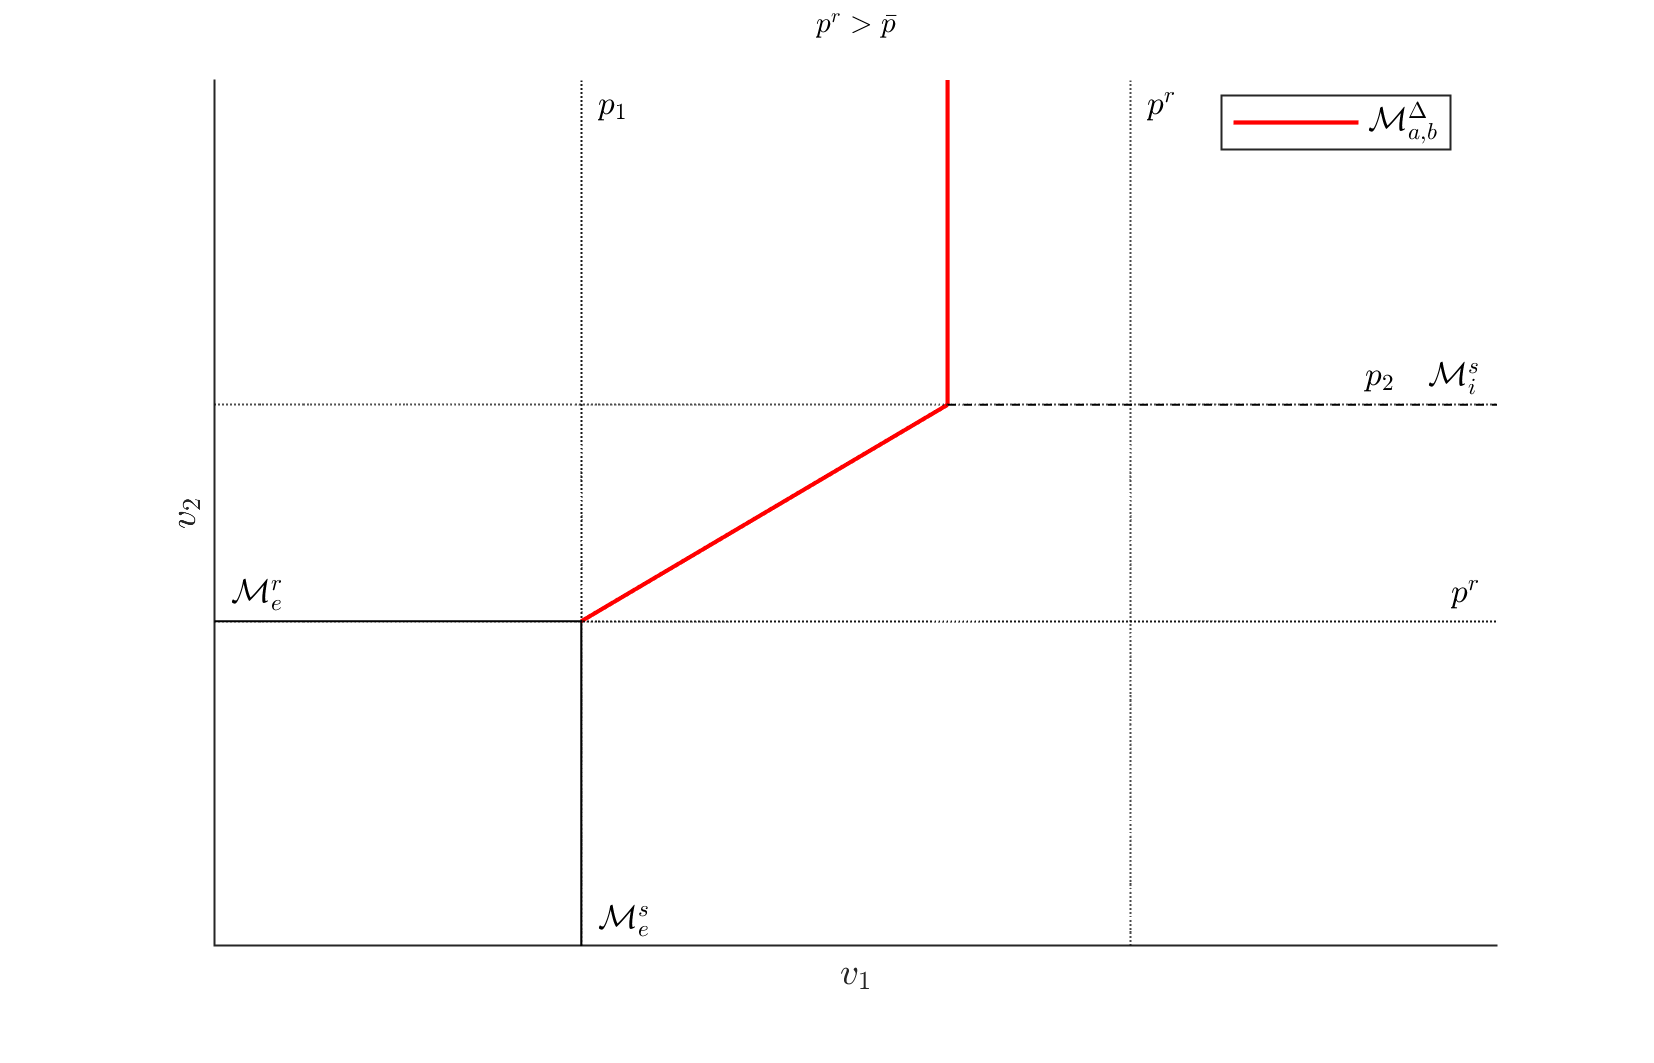
\includegraphics[width=1\linewidth]{figure/example_cstc_ppt1.png}
     \caption{Contract switchers are defined by the red lines.} 
    \label{fig:example_cstc_ppt1}
\end{figure}
    
\end{frame}


%%%%%%%%%%%%%%%%%%%%%%%%%%%%%%%%%%%%%%%%%%%%%%%%%%%%%%%%%%%%%%%%%%%%%%%%%%%%%%%%%%%%%%%%%%%%%%%%%%%%%%%%%%%%%%%%%%%%%%%%%%%%%%%%%%%%%%%%%%%%%%%%%%%%%%

\begin{frame}{The demand for contracts}\label{ExogenousDemand}

\begin{figure}
    \centering
    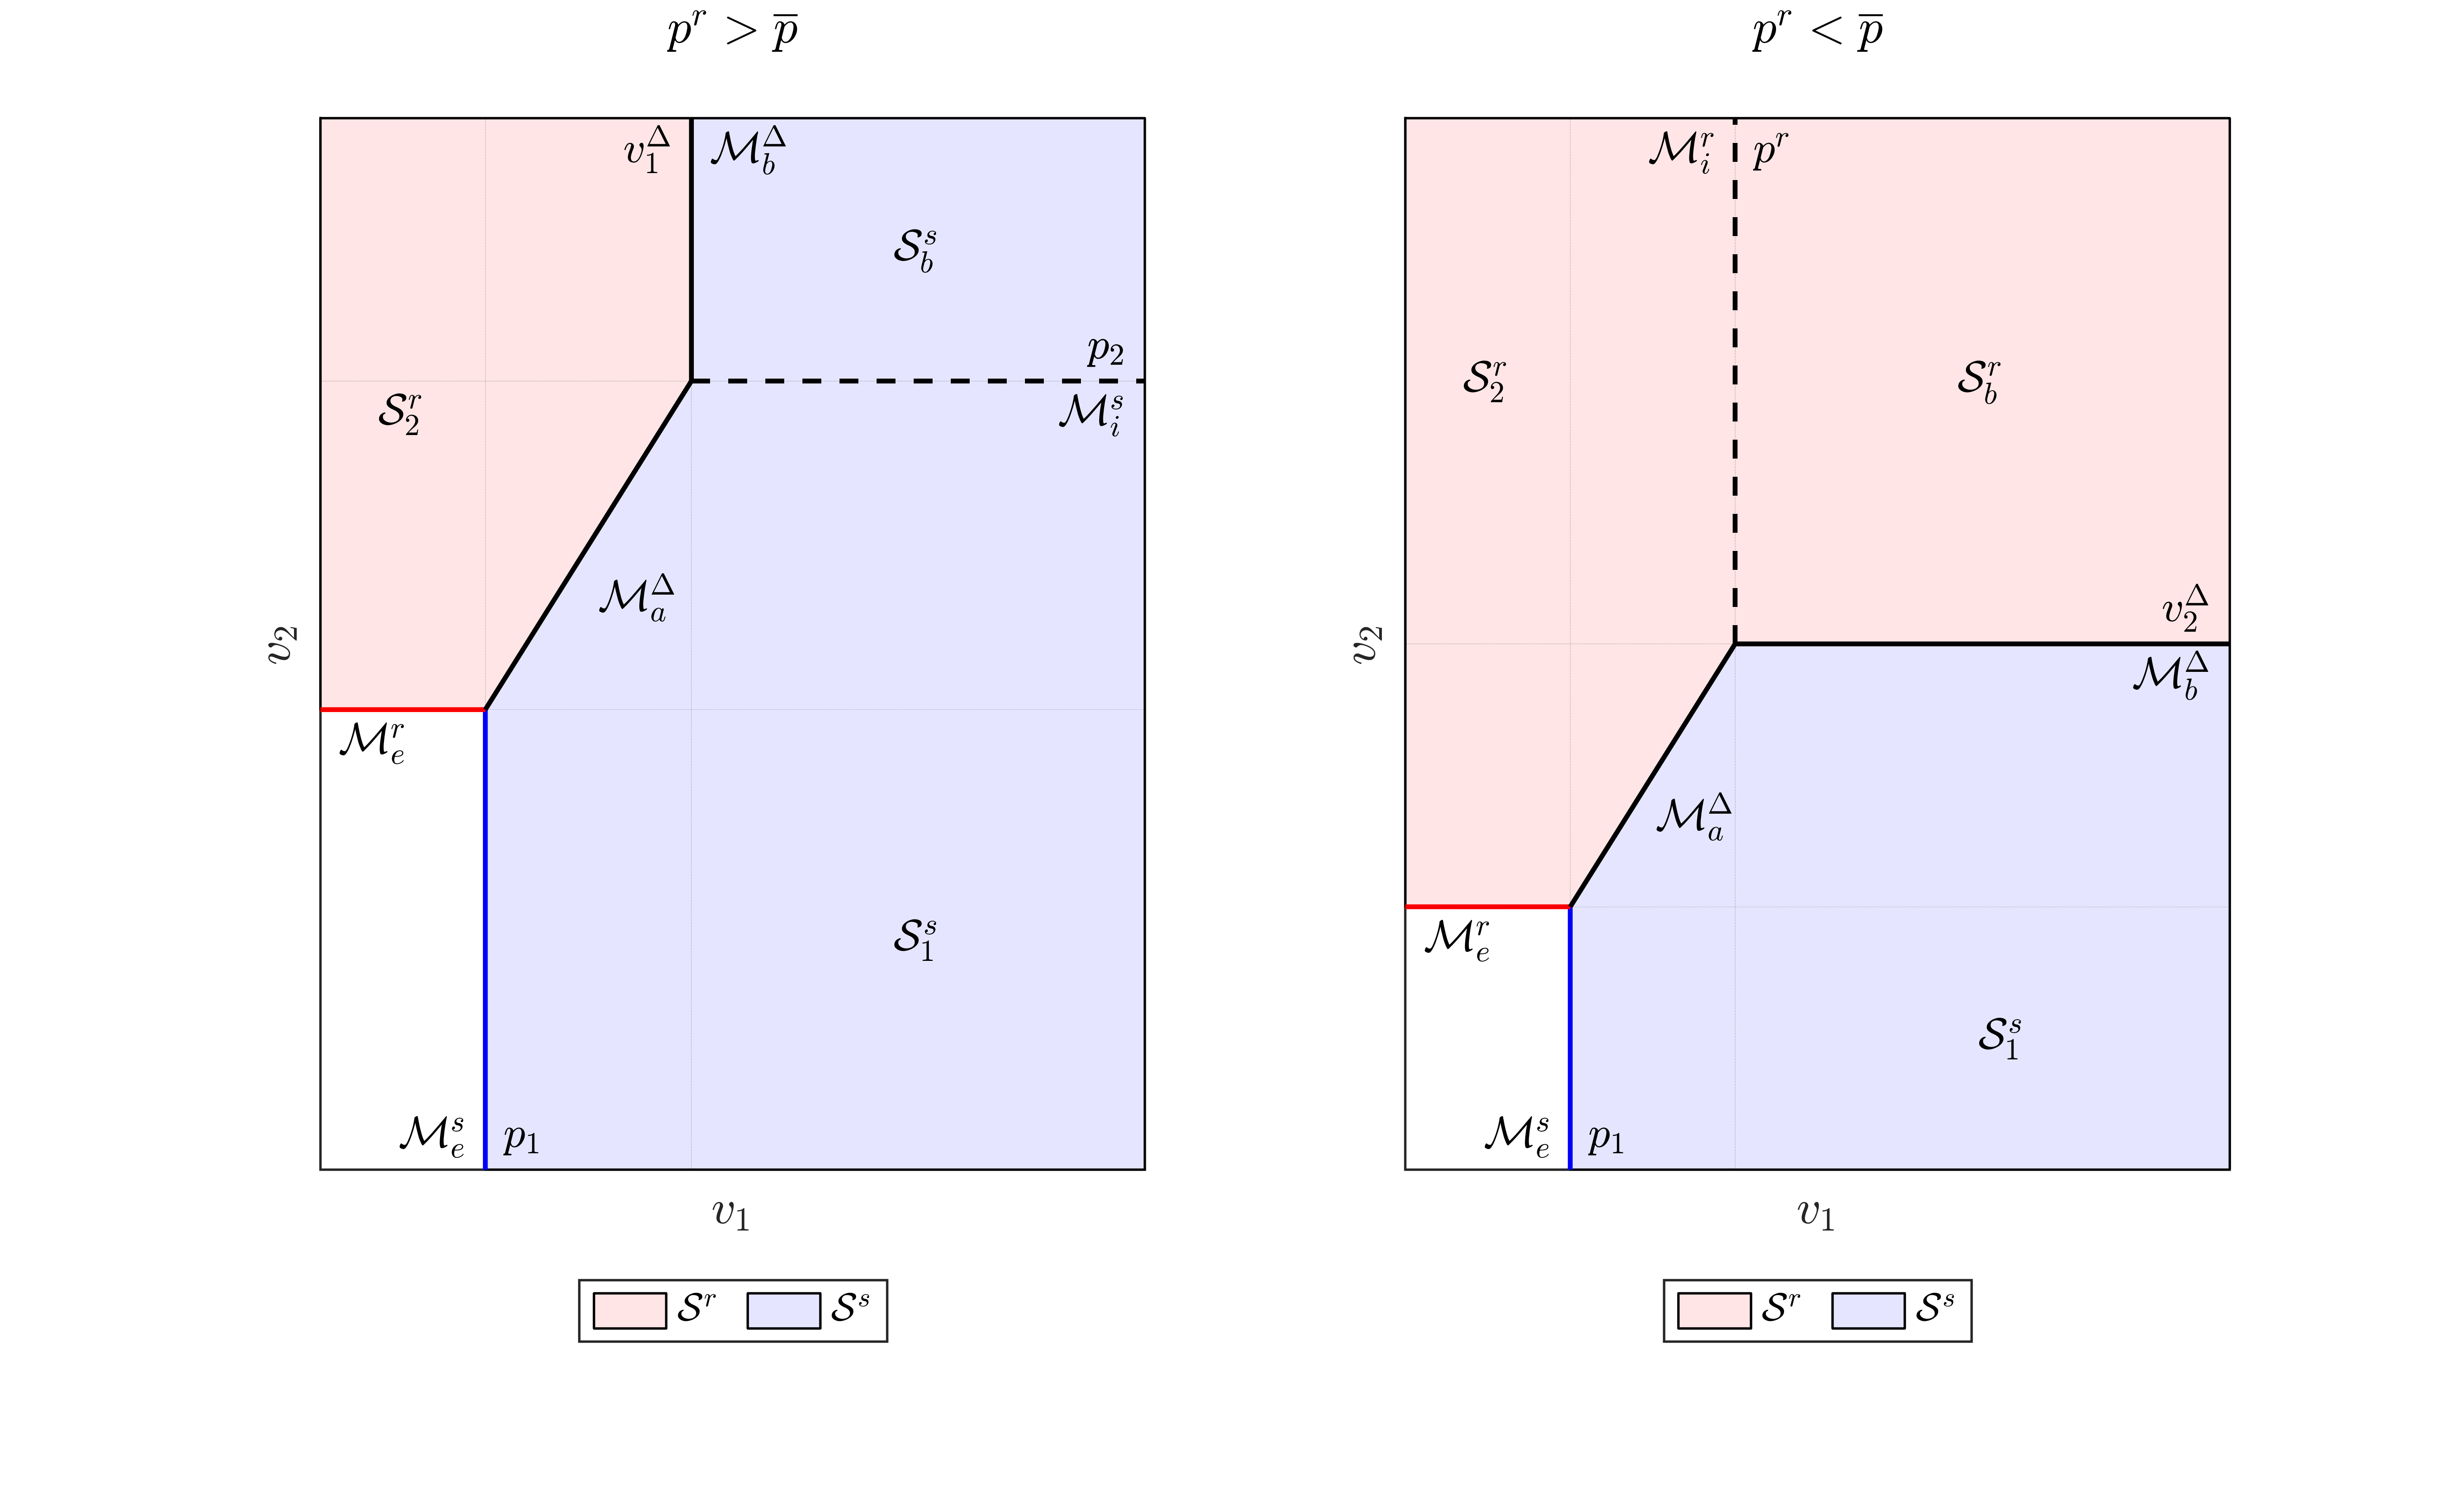
\includegraphics[width=1\linewidth]{figure/example_conv_cstc.png}
     \caption{The set of \textit{contract switchers} defines the mass of consumers choosing each contract.}
\end{figure}
    
\end{frame}


% \begin{frame}{Implication 2: The demand for electricity}\label{ExogenousDemand}

% \begin{figure}
%     \centering
%     \includegraphics[width=1\linewidth]{figure/example_conv_cqtt.png}
%      \caption{When $p^r < \Tilde{p}$ (resp. $p^r > \tilde{p}$ ), some consumers that choose the FP contract (resp. RTP contract) consume in both periods, while consumers under the RTP contracts (resp. FP contract) consume only during period 1 (resp. period 2).}
%     \label{fig:example_conv_cstc4}
% \end{figure}
    
% \end{frame}


%%%%%%%%%%%%%%%%%%%%%%%%%%%%%%%%%%%%%%%%%%%%%%%%%%%%%%%%%%%%%%%%%%%%%%%%%%%%%%%%%%%%%%%%%%%%%%%%%%%%%%%%%%%%%%%%%%%%%%%%%%%%%%%%%%%%%%%%%%%%%%%%%%%%%%
%%%%%%%%%%%%%%%%%%%%%%%%%%%%%%%%%%%%%%%%%%%%%%%%%%%%%%%%%%%%%%%%%%%%%%%%%%%%%%%%%%%%%%%%%%%%%%%%%%%%%%%%%%%%%%%%%%%%%%%%%%%%%%%%%%%%%%%%%%%%%%%%%%%%%%
%%%%%%%%%%%%%%%%%%%%%%%%%%%%%%%%%%%%%%%%%%%%%%%%%%%%%%%%%%%%%%%%%%%%%%%%%%%%%%%%%%%%%%%%%%%%%%%%%%%%%%%%%%%%%%%%%%%%%%%%%%%%%%%%%%%%%%%%%%%%%%%%%%%%%%

% \section{Equilibrium retail prices}

% \begin{frame}{Roadmap}
%   \tableofcontents [sectionstyle=show/shaded,subsectionstyle=show/shaded]
% \end{frame}

%%%%%%%%%%%%%%%%%%%%%%%%%%%%%%%%%%%%%%%%%%%%%%%%%%%%%%%%%%%%%%%%%%%%%%%%%%%%%%%%%%%%%%%%%%%%%%%%%%%%%%%%%%%%%%%%%%%%%%%%%%%%%%%%%%%%%%%%%%%%%%%%%%%%%%



\begin{frame}{Entry of a fixed-price contract}

\begin{figure}
    \centering
    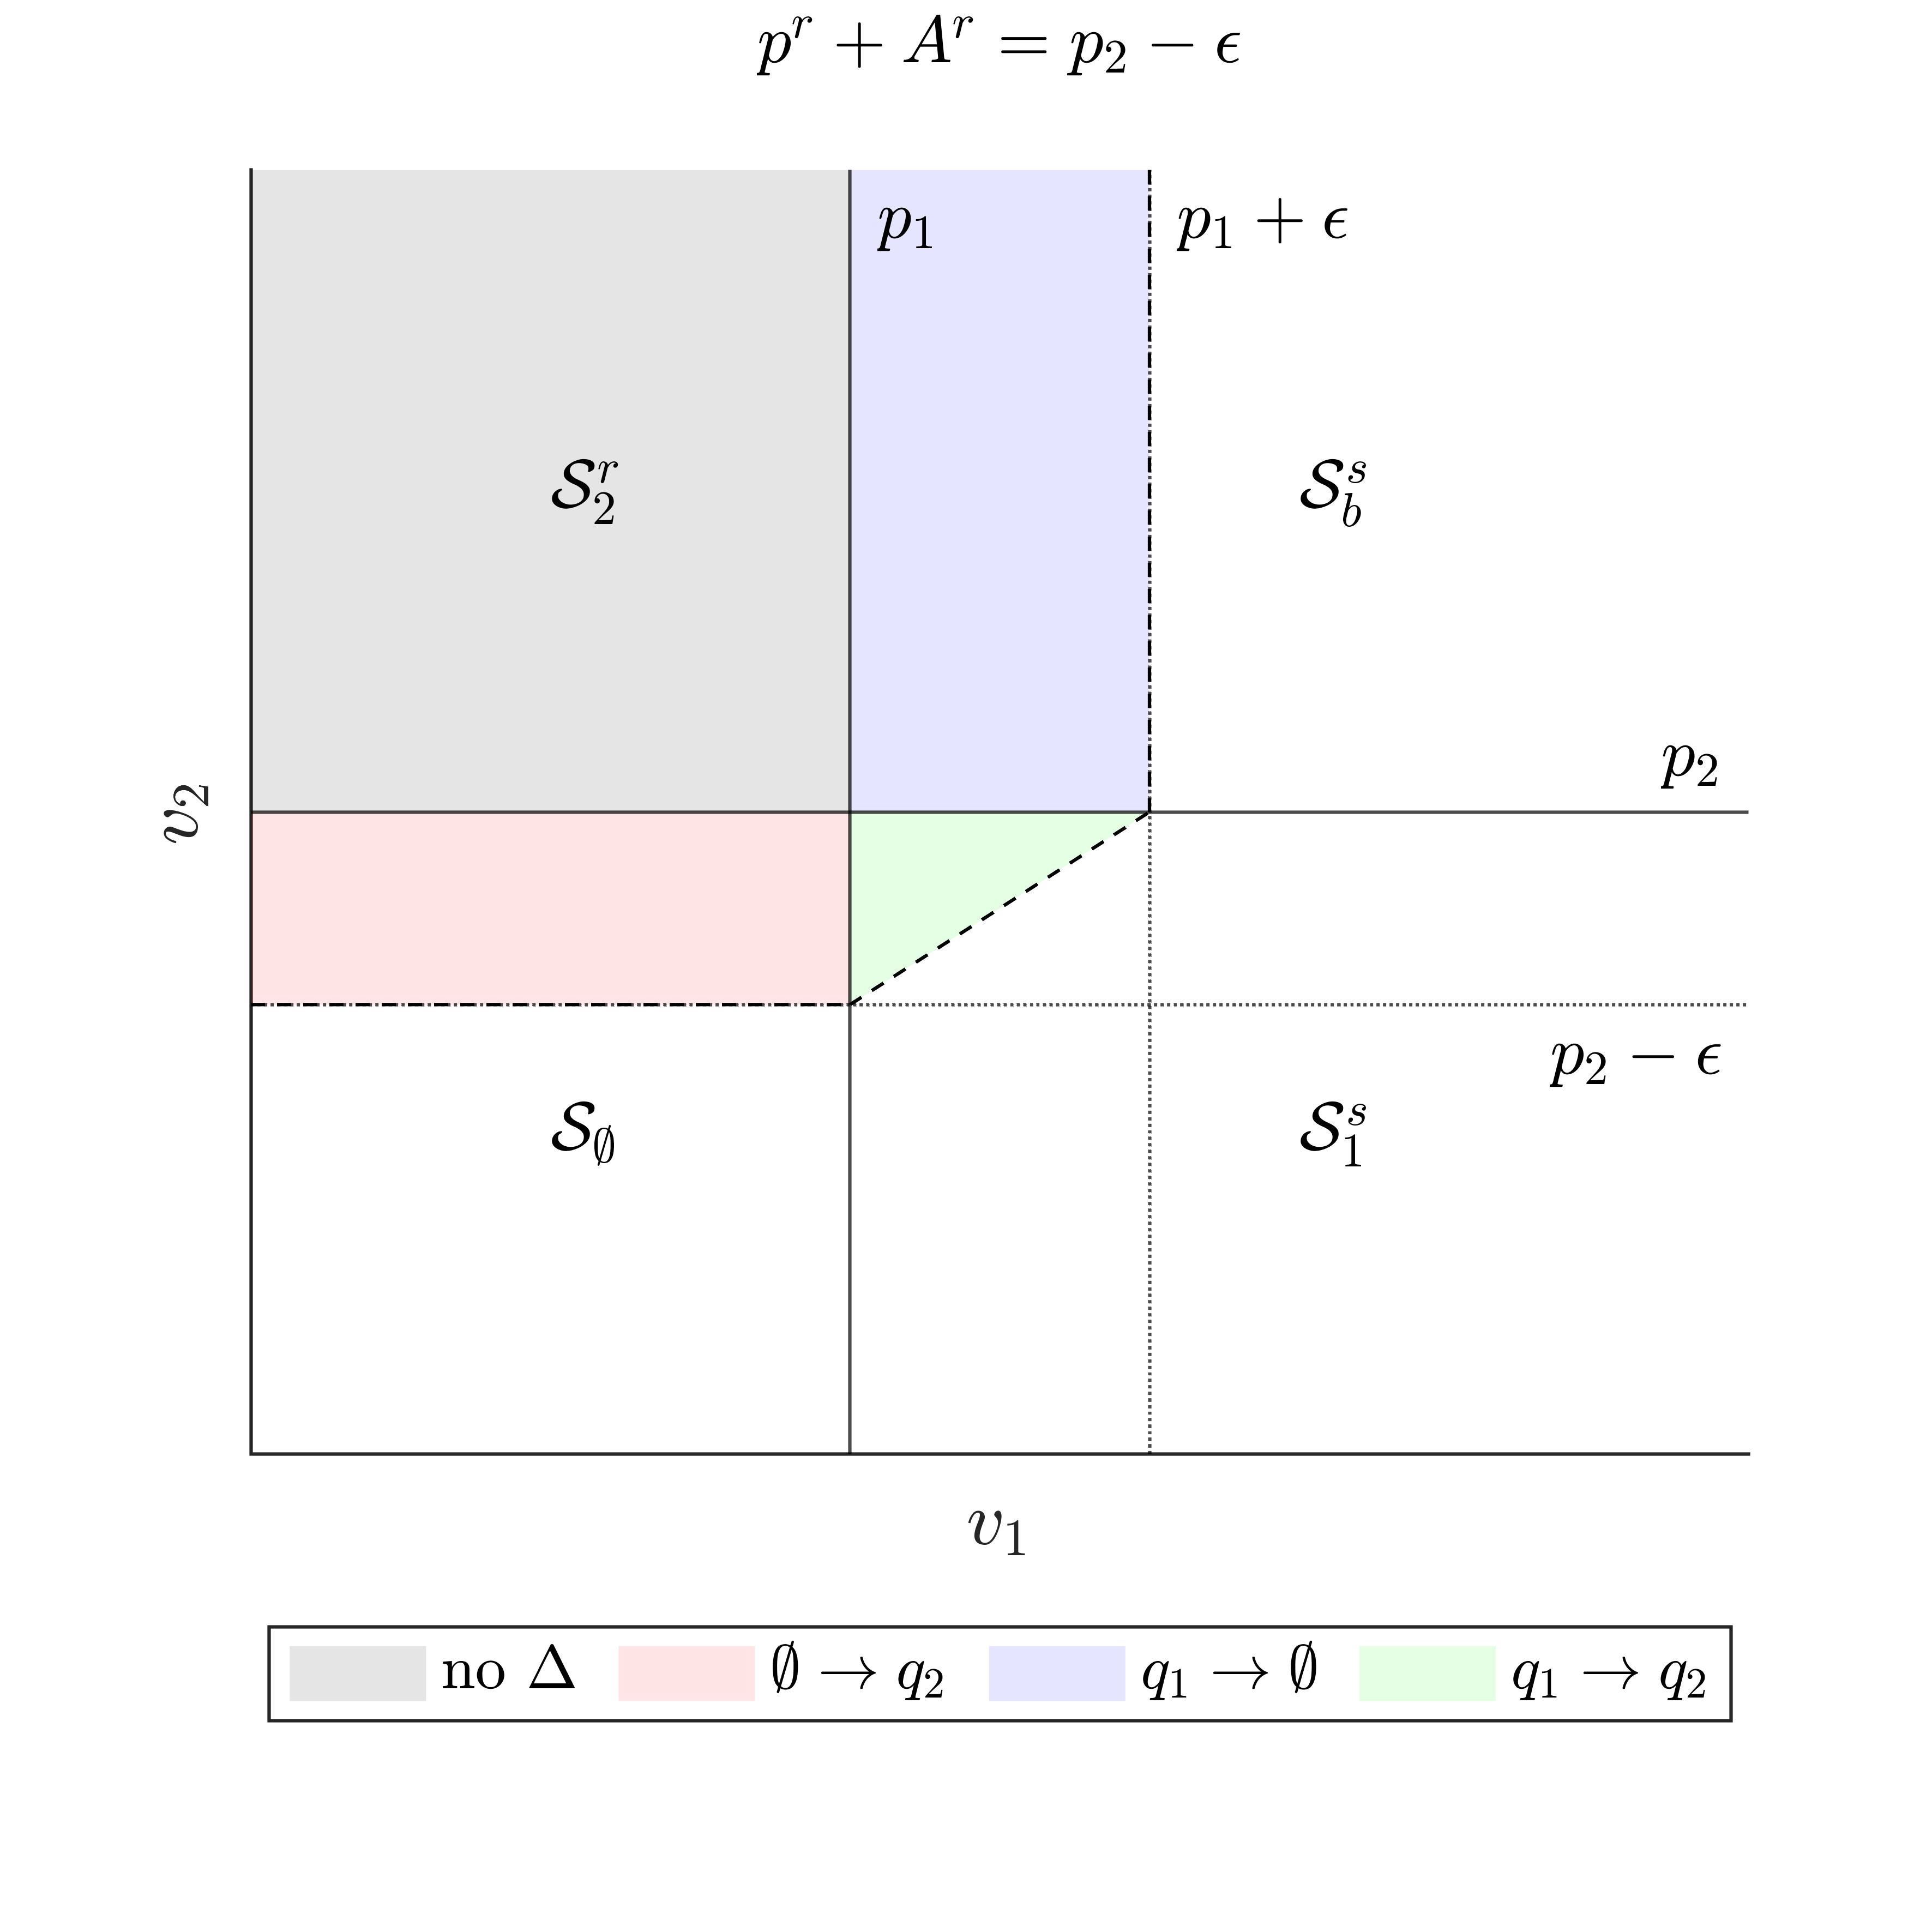
\includegraphics[width=0.65\linewidth]{figure/spot_demand_multi_sb_ppt.png}
    \caption{Downward price deviation of the fixed price with entry.}
    \label{fig:spot_demand_multi_sb_ppt}
\end{figure}
    
\end{frame}

%%%%%%%%%%%%%%%%%%%%%%%%%%%%%%%%%%%%%%%%%%%%%%%%%%%%%%%%%%%%%%%%%%%%%%%%%%%%%%%%%%%%%%%%%%%%%%%%%%%%%%%%%%%%%%%%%%%%%%%%%%%%%%%%%%%%%%%%%%%%%%%%%%%%%%

\begin{frame}{Private firms and self financing-public firm}


\begin{proposition}
     A mixed-equilibrium contract in which consumers have a strict preference for an FP contract offered by private firms does not exist. The unit-price equilibrium of the RTP contract $\textbf{p}^s$ is at the marginal cost: $p_t = c_t \ \forall t$ and $A^s = 0$.
     \label{prop:MSE_PUPR}
\end{proposition}


\vfill


\begin{lemma}\label{lem:tax}
With a public firm and a full self-financing levy, there is no equilibrium with an active FP contract.
\end{lemma}

\vfill

\begin{itemize}
    \item The dynamic contract option lead the market unravelling of the fixed-price contracts. 
\end{itemize}

\end{frame}
% 
%%%%%%%%%%%%%%%%%%%%%%%%%%%%%%%%%%%%%%%%%%%%%%%%%%%%%%%%%%%%%%%%%%%%%%%%%%%%%%%%%%%%%%%%%%%%%%%%%%%%%%%%%%%%%%%%%%%%%%%%%%%%%%%%%%%%%%%%%%%%%%%%%%%%%%

\begin{frame}{Market unraveling of the fixed-price market} \label{PrivateFirms2}


\begin{figure}
    \centering
    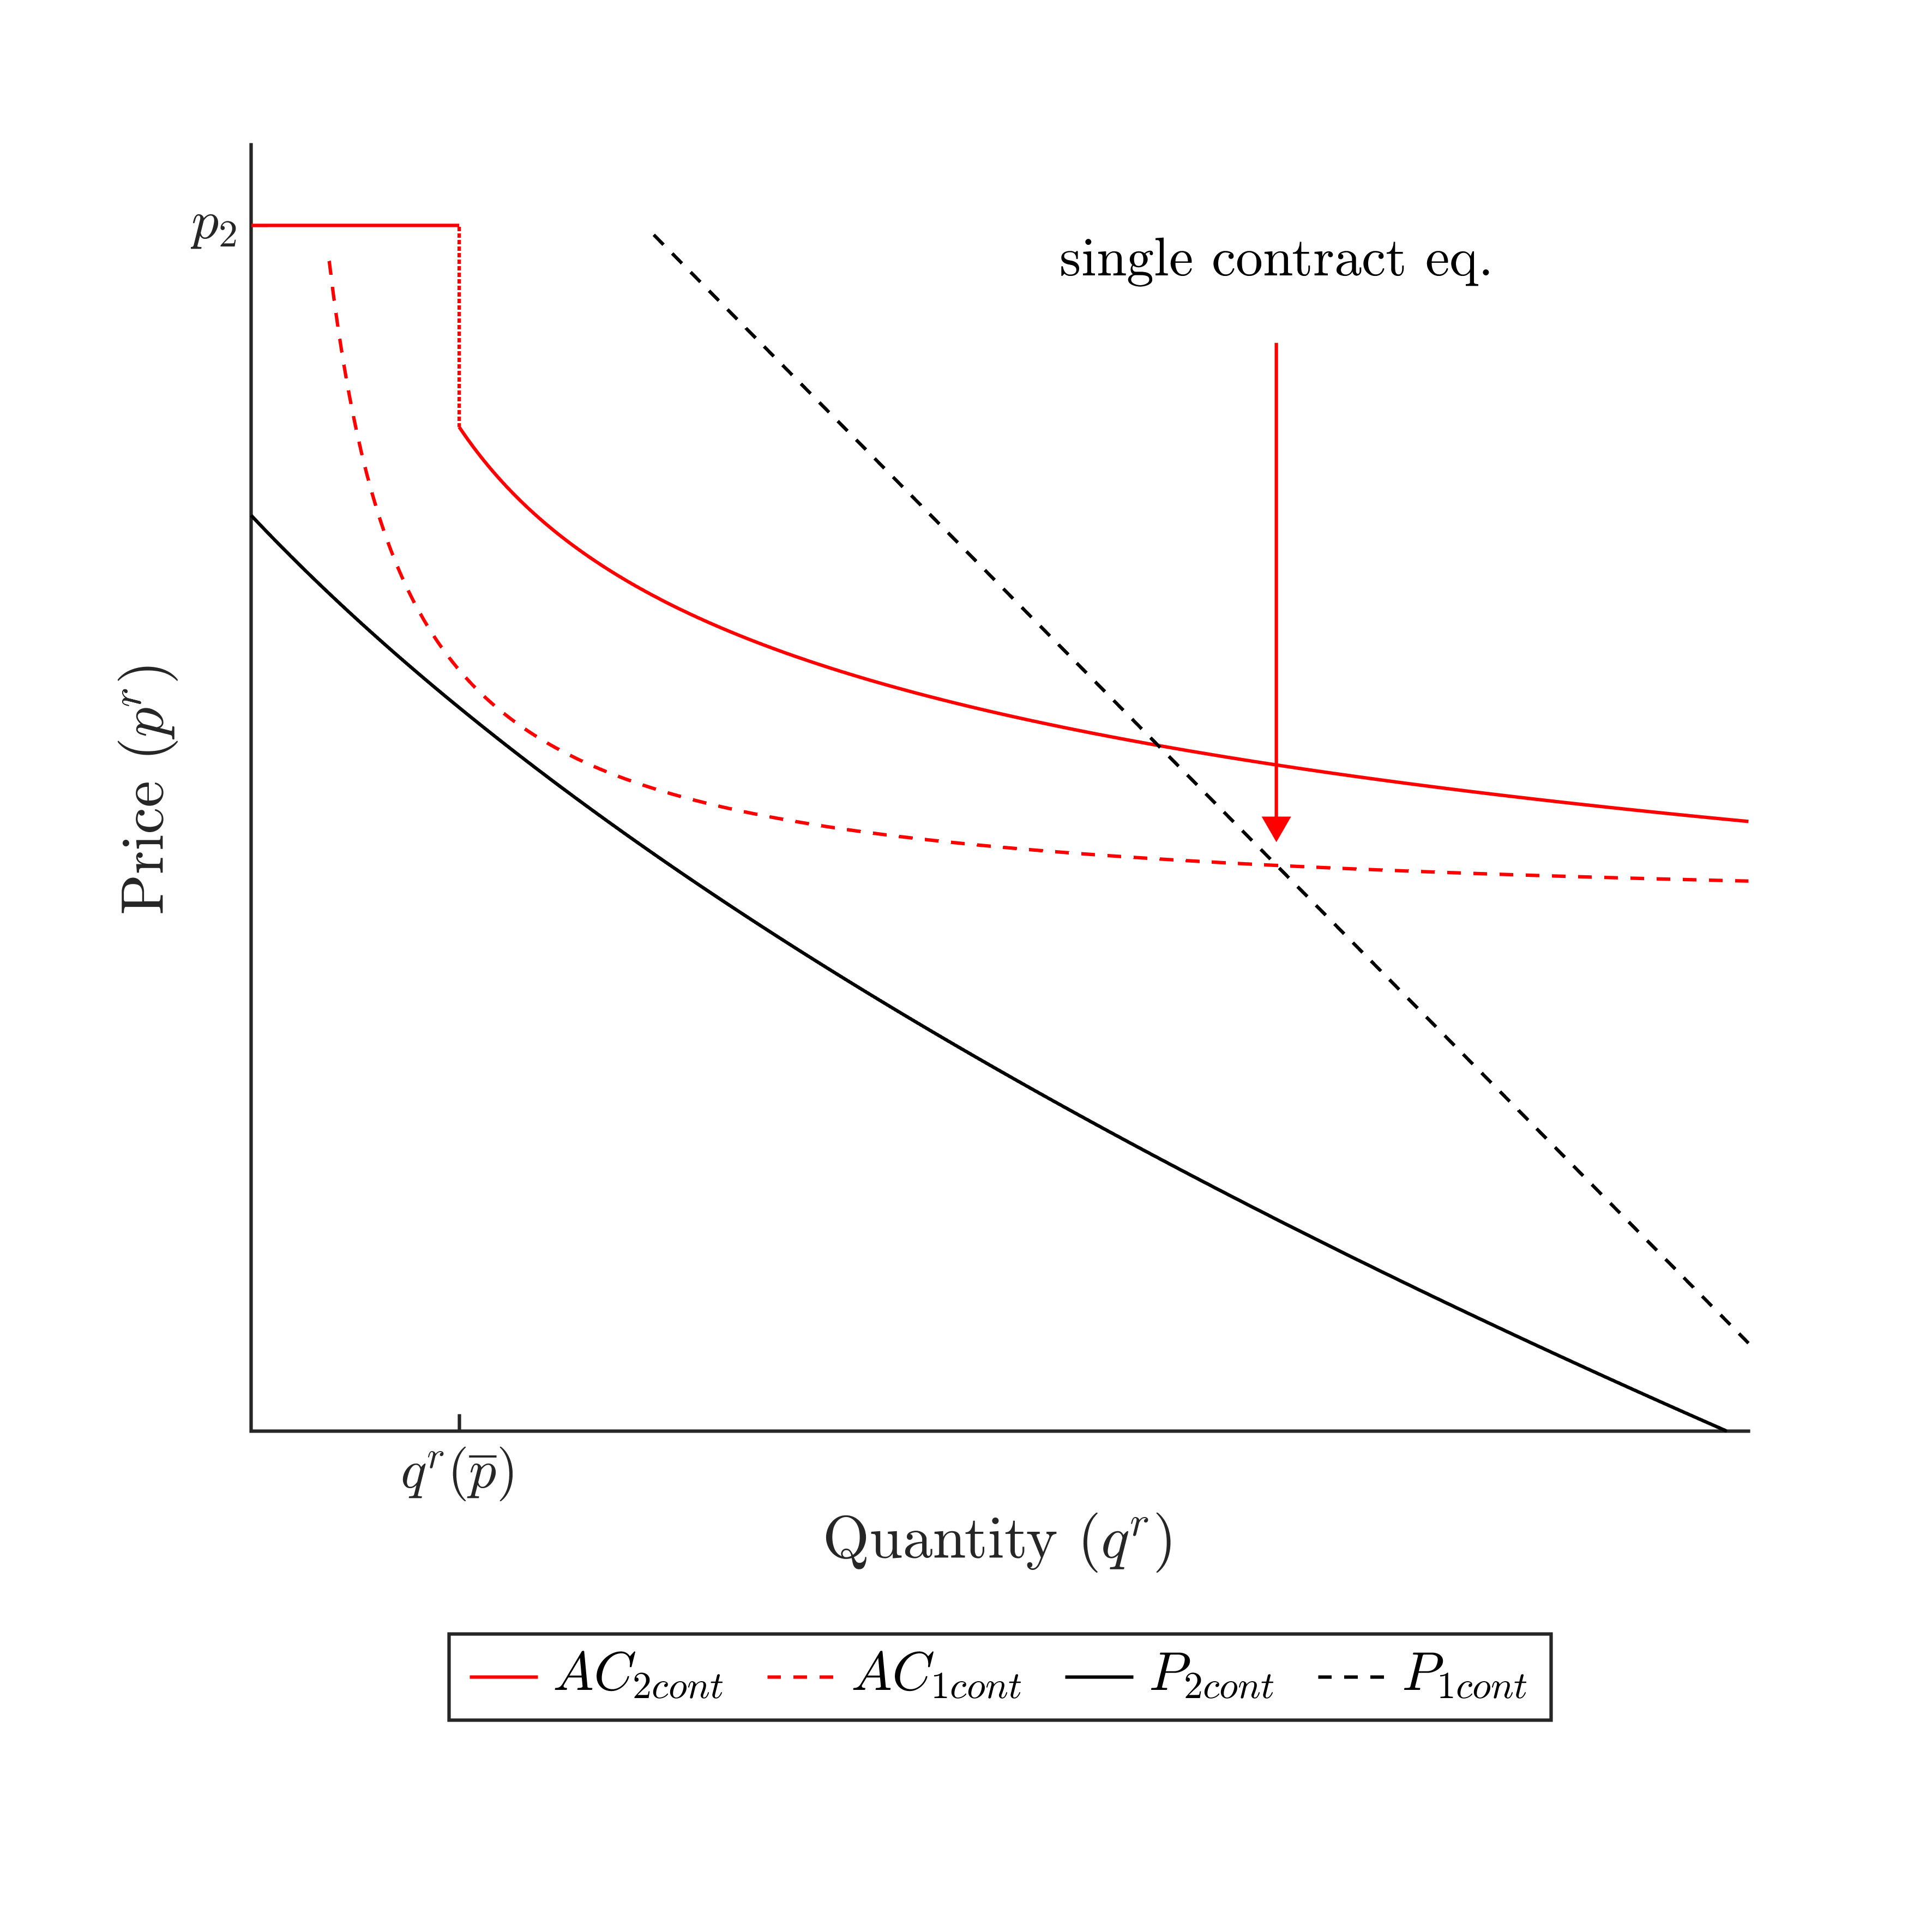
\includegraphics[width=0.75\linewidth]{figure/Exemple_Private_u_ddeAC_ppt.png}
\end{figure}
    
\end{frame}
% 
%%%%%%%%%%%%%%%%%%%%%%%%%%%%%%%%%%%%%%%%%%%%%%%%%%%%%%%%%%%%%%%%%%%%%%%%%%%%%%%%%%%%%%%%%%%%%%%%%%%%%%%%%%%%%%%%%%%%%%%%%%%%%%%%%%%%%%%%%%%%%%%%%%%%%%

\begin{frame}{Public firm price equilibrium}\label{RamseyOutside}

Assume general objective function $CS^r + (1+\lambda) \pi^r$

\vfill

\begin{proposition}\label{prop:sufficientcod}
A public firm has a strict incentive to offer a fixed price contract if: 

\begin{equation*}
    \underbrace{\Bigg. \int_{\M^\Delta|_{\epsilon = 0^+}} (v_2 - p_2) f_1(p_1 ) f_2(v_2 ) dv_2\Bigg.  }_{\text{marginal benefit}} > \underbrace{\Bigg. \lambda q^r|_{\epsilon = 0^+}\Bigg. }_{\text{inframarginal cost}}  \label{con_exi_FP}
\end{equation*}

\end{proposition}

\vfill


\begin{proposition}\label{prop:eqFPPublic}
If an interior equilibrium exists, the unit price $p^r$ and fixed part $A^r$ of the FP contract offered by the public firm satisfy
\begin{equation*}\label{eq1}
p^r\;-\; \text{marginal cost}\;=\; \text{Ramsey terms} \;-\; \underbrace{\Bigg. \frac{1}{1+\lambda}\,\frac{\delta_{A}(\mathcal{C})}{\delta_{A}(q^r)} \Bigg.}_{\text{sorting correction}}
\end{equation*}

\end{proposition}



\end{frame}
%%%%%%%%%%%%%%%%%%%%%%%%%%%%%%%%%%%%%%%%%%%%%%%%%%%%%%%%%%%%%%%%%%%%%%%%%%%%%%%%%%%%%%%%%%%%%%%%%%%%%%%%%%%%%%%%%%%%%%%%%%%%%%%%%%%%%%%%%%%%%%%%%%%%%%

% \begin{frame}{With the regulated monopoly }\label{RamseyMonopoly}


% \begin{itemize}
%     \item We assume that the public firm relies on two sources of financing:  \vfill
%     \begin{itemize}
%         \item The profit from the regulated fixed-price contract.  \vfill
%         \item Unitary tax $t$ levied on all electricity consumers. \vfill
%     \end{itemize}
% \end{itemize}

% \begin{result}

% \vspace{0.1cm}

% There exist some consumers who strictly prefer the FP contract. The full price ($p^r+t_r$) set by the firm solves the following:
 
% \begin{equation*}
%  p^r^{**} \; = p^r^{**} +t_r^{**} \;  = \;  \text{av.marg.cost} \; + \; \text{ramsey}  \; - \;   \underbrace{\bigg. \Omega \bigg.}_{\text{foregone CS}} \; - \;   \underbrace{ \bigg. T \bigg.}_{\text{levy effect}}  
% \end{equation*}

% \end{result}

% \begin{itemize}
%     \item  $T$ = marginal revenue of the tax from the private consumers
%     \item  $\Omega$ = welfare of the \textit{contract switchers}
% \end{itemize}




% \end{frame}

% %%%%%%%%%%%%%%%%%%%%%%%%%%%%%%%%%%%%%%%%%%%%%%%%%%%%%%%%%%%%%%%%%%%%%%%%%%%%%%%%%%%%%%%%%%%%%%%%%%%%%%%%%%%%%%%%%%%%%%%%%%%%%%%%%%%%%%%%%%%%%%%%%%%%%%

% \begin{frame}{Incentive for fixed-price contract}

% \begin{figure}
%     \centering
%     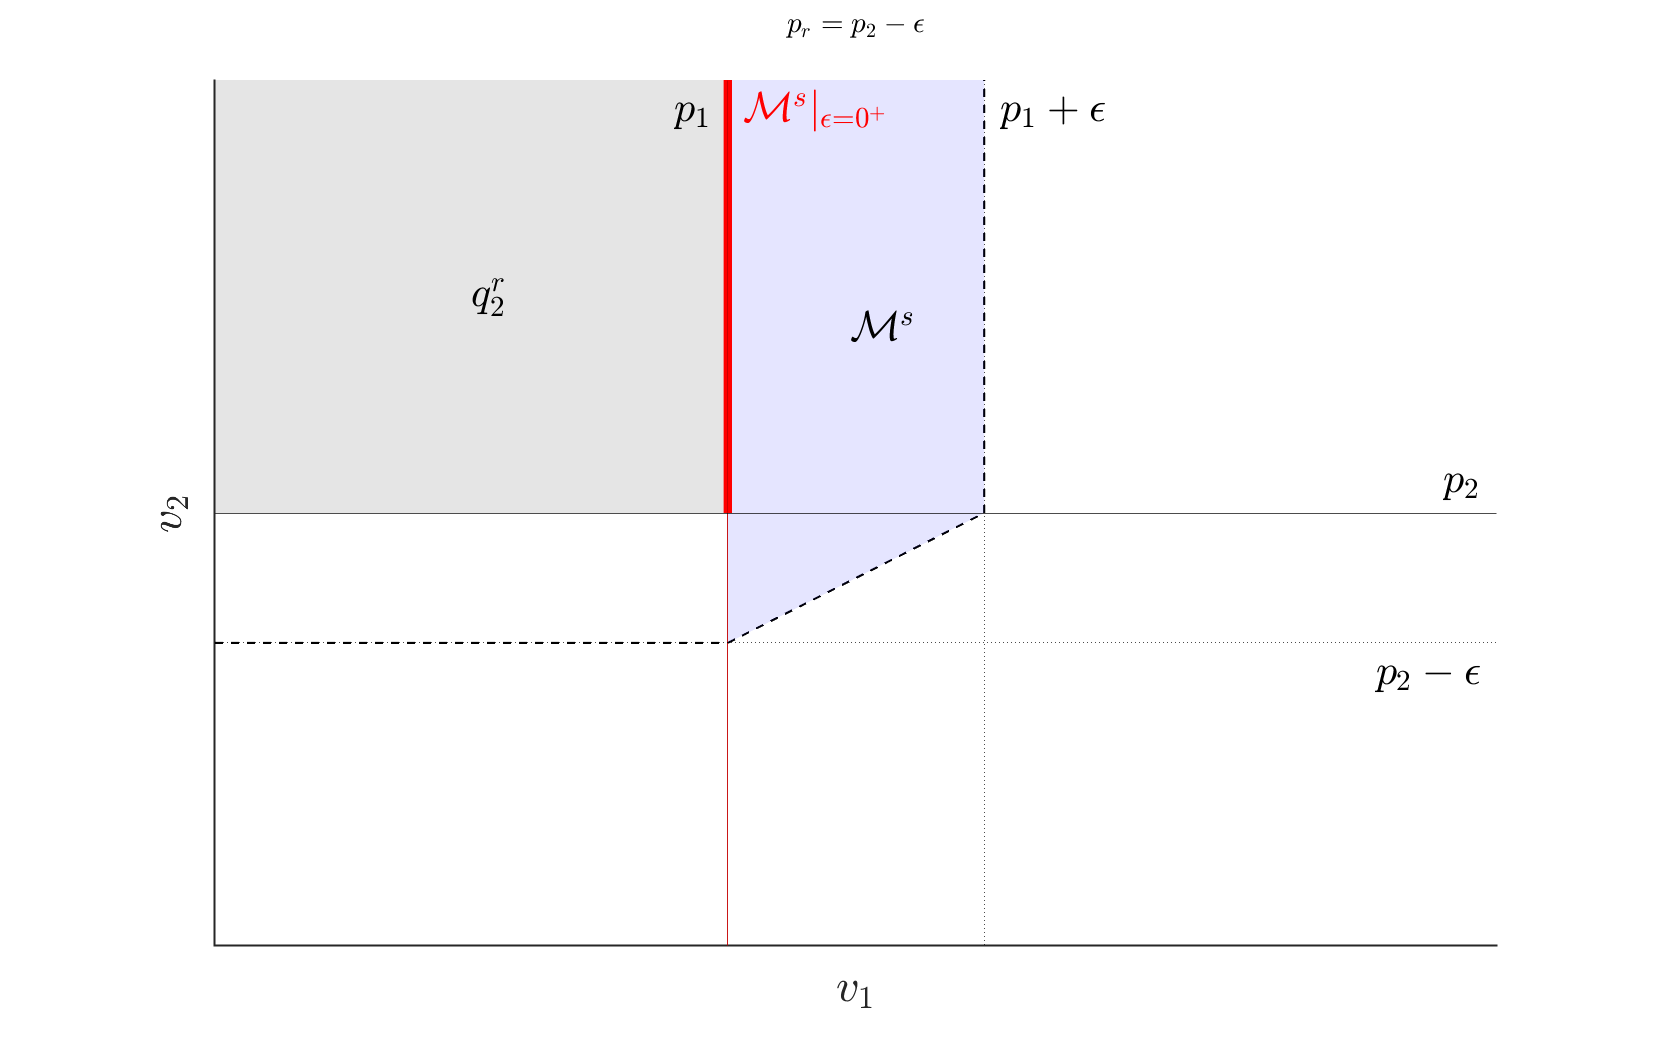
\includegraphics[width=1\linewidth]{figure/spot_demand_multi_sb_ppt_equil.png}
%     \caption{Tradeoff for profitability of the public fixed-price contract.}
%     \label{fig:spot_demand_multi_sb_ppt_equil}
% \end{figure}
    
% \end{frame}

%%%%%%%%%%%%%%%%%%%%%%%%%%%%%%%%%%%%%%%%%%%%%%%%%%%%%%%%%%%%%%%%%%%%%%%%%%%%%%%%%%%%%%%%%%%%%%%%%%%%%%%%%%%%%%%%%%%%%%%%%%%%%%%%%%%%%%%%%%%%%%%%%%%%%%

\begin{frame}{Illustration of $\mathcal{C}$}

\begin{figure}
    \centering
    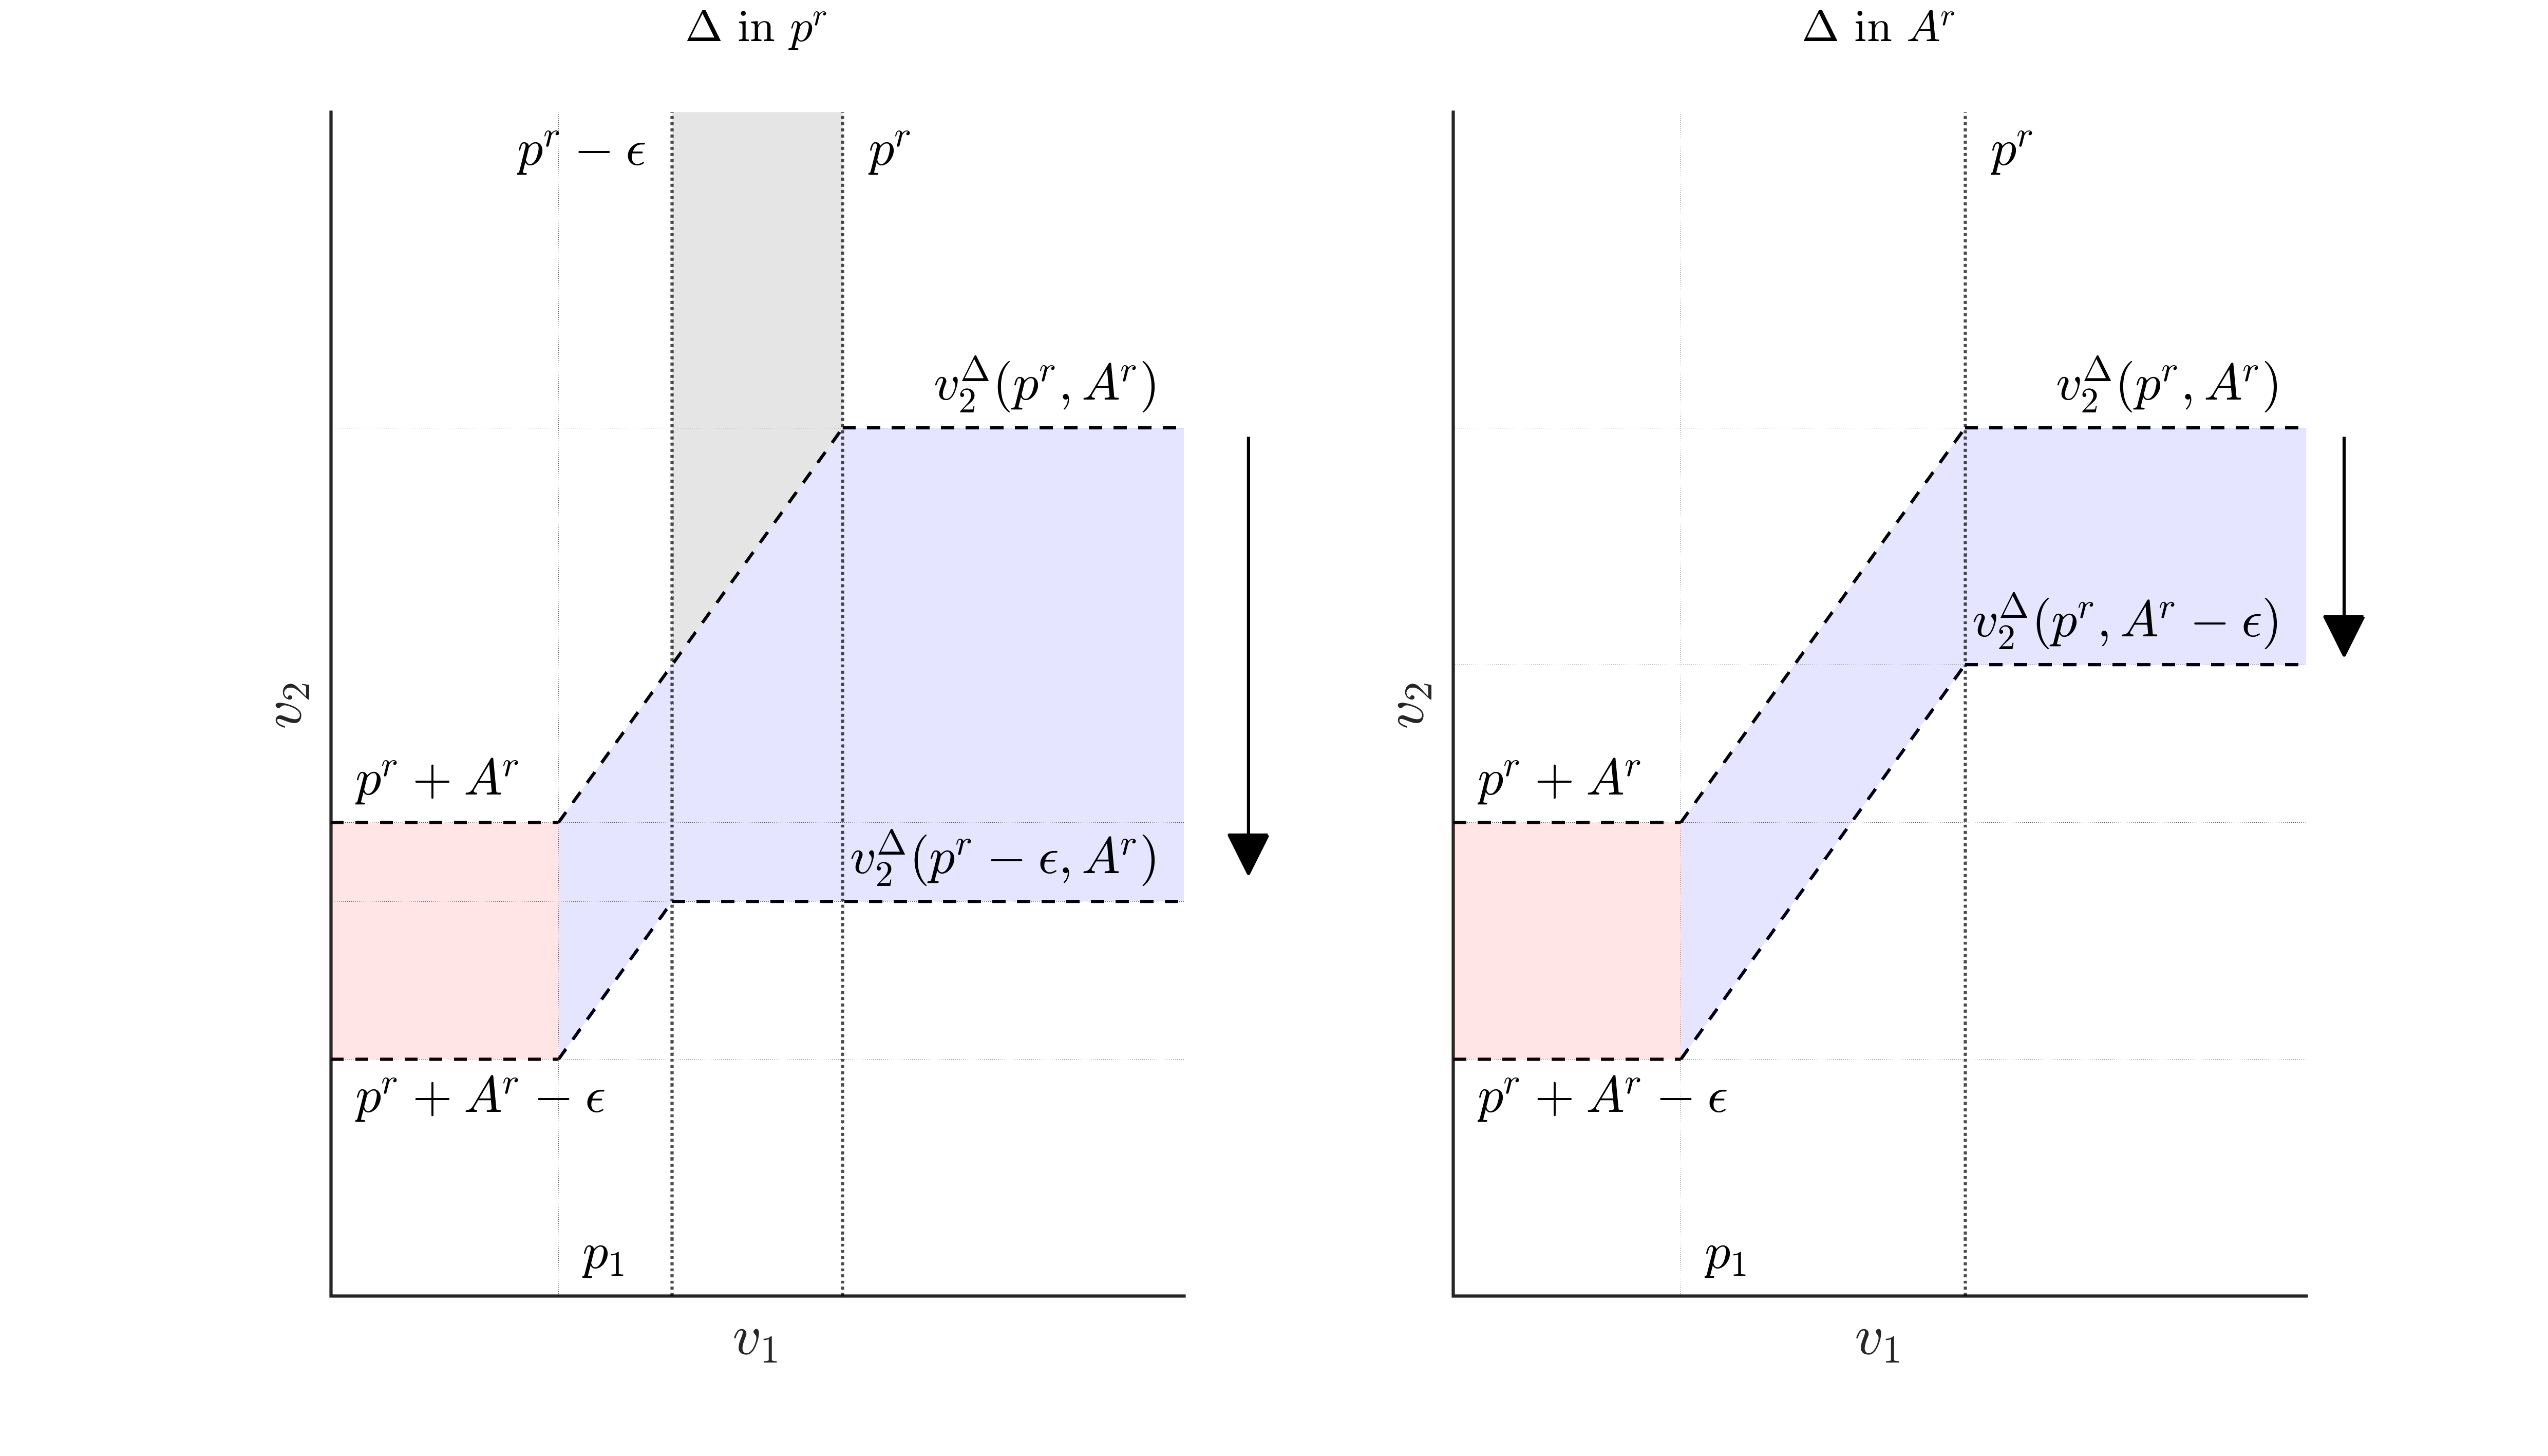
\includegraphics[width=1\linewidth]{figure/spot_demand_v2_sb_ppt.png}
    \caption{$\mathcal{C}$ captures the (marginal) consumer surplus lost to the private firms.}
    \label{fig:spot_demand_v2_sb_ppt}
\end{figure}
    
\end{frame}

%%%%%%%%%%%%%%%%%%%%%%%%%%%%%%%%%%%%%%%%%%%%%%%%%%%%%%%%%%%%%%%%%%%%%%%%%%%%%%%%%%%%%%%%%%%%%%%%%%%%%%%%%%%%%%%%%%%%%%%%%%%%%%%%%%%%%%%%%%%%%%%%%%%%%%

\section{Welfare Implications}

%%%%%%%%%%%%%%%%%%%%%%%%%%%%%%%%%%%%%%%%%%%%%%%%%%%%%%%%%%%%%%%%%%%%%%%%%%%%%%%%%%%%%%%%%%%%%%%%%%%%%%%%%%%%%%%%%%%%%%%%%%%%%%%%%%%%%%%%%%%%%%%%%%%%%%

% \begin{frame}{Roadmap}
%   \tableofcontents [sectionstyle=show/shaded,subsectionstyle=show/shaded]
% \end{frame}

%%%%%%%%%%%%%%%%%%%%%%%%%%%%%%%%%%%%%%%%%%%%%%%%%%%%%%%%%%%%%%%%%%%%%%%%%%%%%%%%%%%%%%%%%%%%%%%%%%%%%%%%%%%%%%%%%%%%%%%%%%%%%%%%%%%%%%%%%%%%%%%%%%%%%%

\begin{frame}{Welfare comparison}


\begin{itemize}
   
    \item Only private firms: \boldrblue{ First-Best}. \vfill

    \item Public Firm + Private Firms + Consumer Choices \boldrblue{?} \vfill

    \item We compare the welfare with \boldrblue{a single contract} environment. \vfill

    \begin{itemize}
        \item We show that the \boldrblue{welfare can be ambiguous}. \vfill
        \item This is notably due to having \boldrblue{a lower fixed-price} compared to the single contract case.
    \end{itemize}
    
\end{itemize}
    
\end{frame}

\begin{frame}{Deadweight loss with FP contracts}
    \begin{figure}
        \centering
        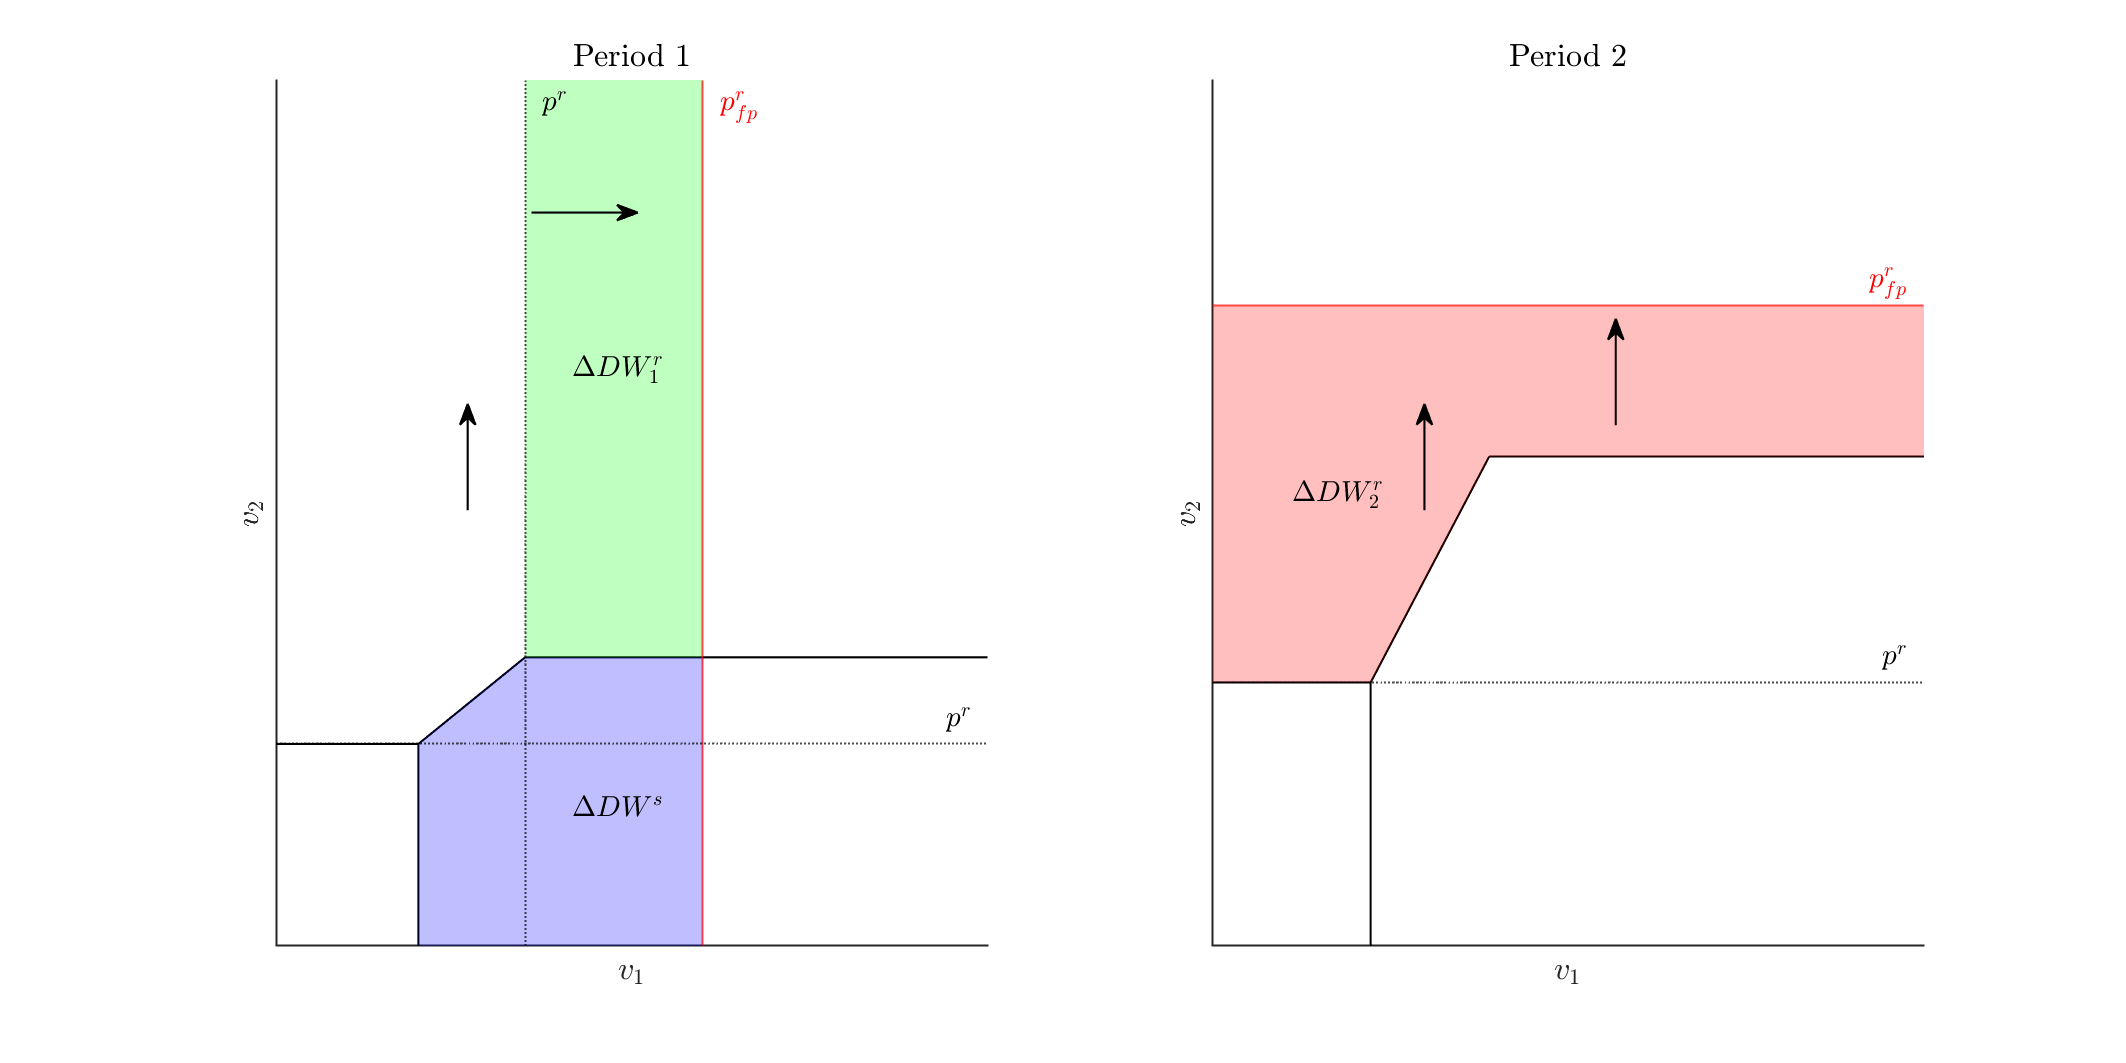
\includegraphics[width=1.0\linewidth]{figure/ExampleSurplusCUNIF.png}
        \caption{$p^r$ is the equilibrium with consumer choice and $p^r_{fp}$ is the equilibrium with only FP contract}
        \label{fig:ExampleSurplusCUNIF}
    \end{figure}
\end{frame}


\begin{frame}{Self-Selection Equilibrium vs. S.B. Linear Pricing FP Contract }

\begin{figure}
    \centering
    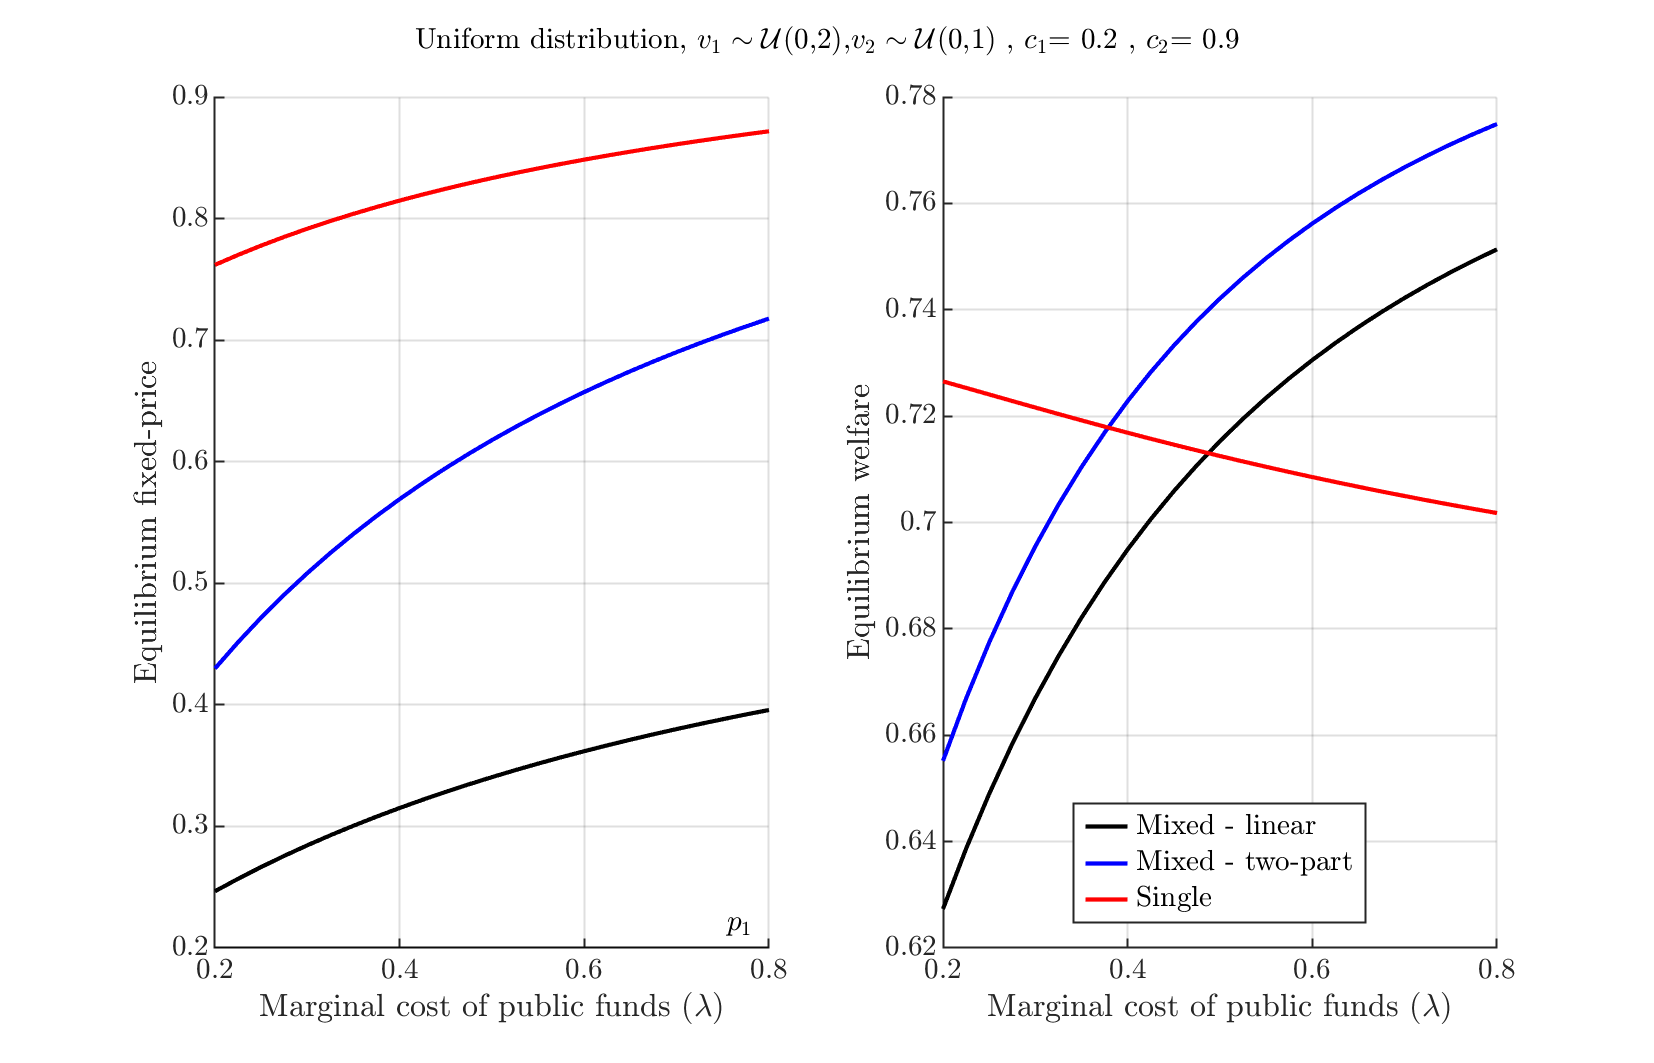
\includegraphics[width=0.9\linewidth]{figure/example_equ0_PublicFund_u.png}
        \caption{$W = CS + \Pi$.}
\end{figure}
    
\end{frame}


%%%%%%%%%%%%%%%%%%%%%%%%%%%%%%%%%%%%%%%%%%%%%%%%%%%%%%%%%%%%%%%%%%%%%%%%%%%%%%%%%%%%%%%%%%%%%%%%%%%%%%%%%%%%%%%%%%%%%%%%%%%%%%%%%%%%%%%%%%%%%%%%%%%%%%

\begin{frame}{Application - Consumer distribution}

\begin{figure}
    \centering
    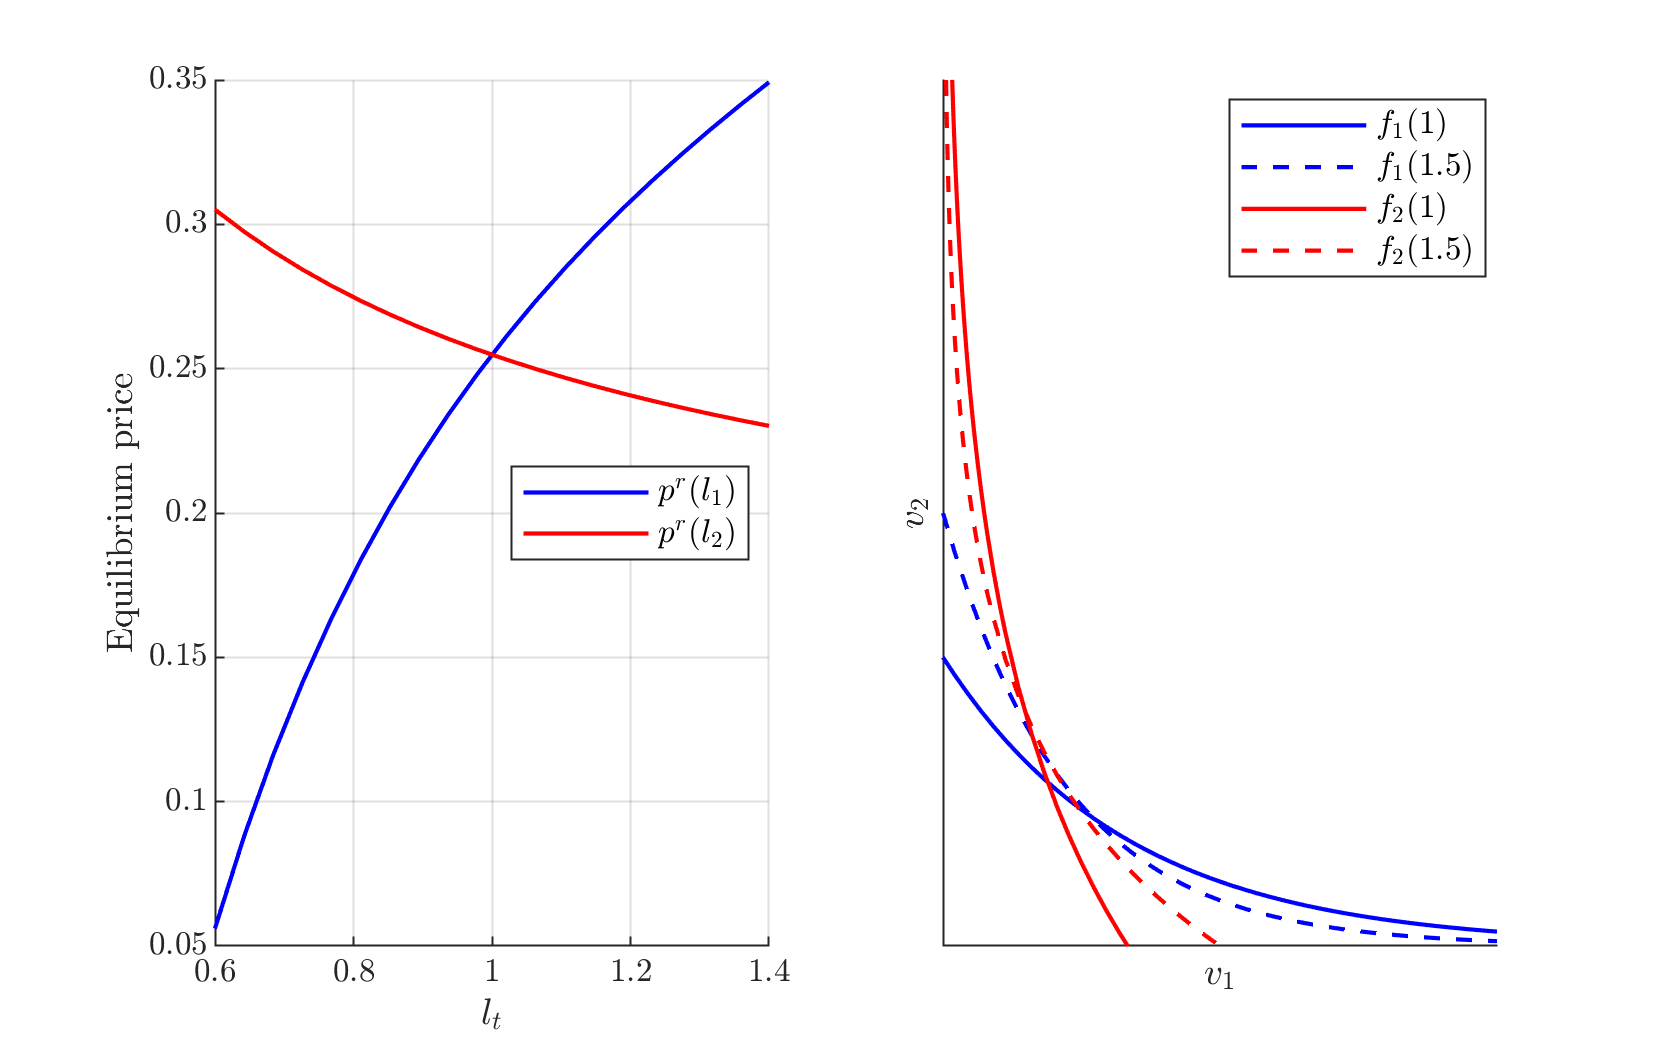
\includegraphics[width=0.95\linewidth]{figure/example_pdfeq.png}
    \caption{Exponential distribution: $v_t\sim \mathrm{Exp}(l_t)$ with $l_t>0$}
\end{figure}
    
\end{frame}

%%%%%%%%%%%%%%%%%%%%%%%%%%%%%%%%%%%%%%%%%%%%%%%%%%%%%%%%%%%%%%%%%%%%%%%%%%%%%%%%%%%%%%%%%%%%%%%%%%%%%%%%%%%%%%%%%%%%%%%%%%%%%%%%%%%%%%%%%%%%%%%%%%%%%%


\section{Conclusion}



\begin{frame}{Conclusion}

\begin{itemize}
    \item The paper provides a novel framework describing the self-selection of electricity contracts by heterogeneous consumers.\vfill
    \item We show that the coexistence of a public option with a private sector and self-selection from consumers can lead to low welfare due to adverse selection. \vfill
    \item Going beyond the impossibility result: How to make the curves cross?  \vfill
    \begin{itemize}
        \item Different selection pattern: risk aversion. \vfill
        \item Barrier to selection: $p^r > AC(p^r)$. \vfill
        \item Lower retail cost: $\overline{AC}(p^r)<AC(p^r)$.
    \end{itemize}
    \vfill 
    \item Sophisticated firms: price discrimination $\approx$ public firm? 
\end{itemize}
    
\end{frame}



% \end{document}


%%%%%%%%%%%%%%%%%%%%%%%%%%%%%%%%%%%%%%%%%%%%%%%%%%%%%%%%%%%%%%%%%%%%%%%%%%%%%%%%%%%%%%%%%%%%%%%%%%%%%%%%%%%%%%%%%%%%%%%%%%%%%%%%%%%%%%%%%%%%%%%%%%%%%%


\begin{frame}{}
  \centering {\Huge
  \emph{Thank you !}}
  
  \vspace{1cm}

  http://leopoldmonjoie.com/
\end{frame}




\newcounter{totalbeforeappendix}
\setcounter{totalbeforeappendix}{\value{framenumber}}
\addtocounter{totalbeforeappendix}{2} 
\addtocounter{framenumber}{-9}

\bibliography{bib}

\end{document}

\begin{frame}{Literature: Demand for contracts}\label{Lit_Conso}

\begin{itemize}
    \item \textbf{No theoretical foundation of self-selection in the power retail market}.

    \vfill
    
    \item Variation of an \boldrblue{exogenous share} of RTP consumers.
    \begin{itemize}
        \item Seminal paper: \cite{Borenstein2005b}, Technological cost \cite{Leautier2014},  Interactions with renewable technologies \cite{Ambec2021}, Risk aversion \cite{Boom2021}.
        \item \boldrblue{limits}: single period - homogenous consumers. 
    \end{itemize}

 \vfill

    \item \boldrblue{Empirical evidence} of self-selection with heterogeneous consumers
    \begin{itemize}
        \item Adverse selection \cite{Ito2023} Risk aversion \cite{Qiu2018} Behavioral bias \cite{Hortacsu2017,Fowlie2021}
        \item \boldrblue{limits}: focus on behavioral biais.
    \end{itemize}


\vfill
    \item Empirical evidence of RTP contracts.
    
    \begin{itemize}
        \item Effect of contract prices on consumption \cite{Fabra2021,Han2023,Enrich2024,Fu2024}, Redistributive effect \cite{Leslie2021, Levinson2022a, Cahana2023}
    \end{itemize}


     
    
\end{itemize}

\vfill

\hyperlink{FirstCont}{\beamergotobutton{Back}}

\end{frame}

%%%%%%%%%%%%%%%%%%%%%%%%%%%%%%%%%%%%%%%%%%%%%%%%%%%%%%%%%%%%%%%%%%%%%%%%%%%%%%%%%%%%%%%%%%%%%%%%%%%%%%%%%%%%%%%%%%%%%%%%%%%%%%%%%%%%%%%%%%%%%%%%%%%%%%

\begin{frame}{Literature: Retail competition}\label{Lit_Mkt1}
    
    
\begin{itemize}
    \item \textbf{Little attention on the competition in the retail market and contract equilibrium}.  
    
    \vfill

    \item Few empirical works on the benefit of retail competition \cite{Concettini2013}. Retailers acting as in Bertrand competition \cite{von2010electricity}
    
    \vfill

   \item Seminal papers \cite{joskow2006retail} and \cite{Borenstein2003}. \boldrblue{limits}: homogeneous consumers - simplified market structure.

\vfill

   \item  \boldrblue{Adverse selection} in retail electricity market
   
   \begin{itemize}
       \item Consumers deviation \cite{chao2013incentive}
       \item IC contracts and market equilibrium \cite{Astier2021}
   \end{itemize}

\vfill

    \item \boldrblue{Outside public option with incomplete information}
    \begin{itemize}
        \item In electricity markets with a regulated firm with redistributive preferences \cite{Martimort2020a} in a general setting \cite{Kang2023a}
    \end{itemize}


% \vfill

% \item Market power and price discrimination in retail electricity market \cite{byrne2022price}

\end{itemize}

\vfill



\hyperlink{SecondCont}{\beamergotobutton{Back}}

\end{frame}


%%%%%%%%%%%%%%%%%%%%%%%%%%%%%%%%%%%%%%%%%%%%%%%%%%%%%%%%%%%%%%%%%%%%%%%%%%%%%%%%%%%%%%%%%%%%%%%%%%%%%%%%%%%%%%%%%%%%%%%%%%%%%%%%%%%%%%%%%%%%%%%%%%%%%%

\begin{frame}{Literature: Other litterature }\label{Lit_Mkt2}
    
    
\begin{itemize}

   \item \textbf{Adverse Selection}
   \begin{itemize}
       \item Selection on the level and selection on the slope \cite{Einav2011,Einav2021}
       \item Empirical evidence for electricity contracts \cite{Ito2023}
   \end{itemize}


\vfill

   \item \textbf{Self-Selection}
    \begin{itemize}
        \item Roy Model \cite{Barro2013}
        \item Applied to Energy Efficiency \cite{Allcott2014}
    \end{itemize}

\vfill

   \item \textbf{Durable Goods}
   \begin{itemize}
       \item Household as production unit \cite{Becker1965}
       \item Applied to short-term/long-term decisions \cite{Feger2022} 
   \end{itemize}

\vfill

   \item \textbf{Competition for non-linear contracts}
   \begin{itemize}
       \item General setting \cite{Stole2007}
       \item Applied to insurance \cite{Rothschild1976,Dosis2022} 
   \end{itemize}
   
\vfill

   \item \textbf{Multidimensional Screening} \cite{Rochet1998}
   
\end{itemize}
\vfill

\hyperlink{SecondCont}{\beamergotobutton{Back}}

\end{frame}


%%%%%%%%%%%%%%%%%%%%%%%%%%%%%%%%%%%%%%%%%%%%%%%%%%%%%%%%%%%%%%%%%%%%%%%%%%%%%%%%%%%%%%%%%%%%%%%%%%%%%%%%%%%%%%%%%%%%%%%%%%%%%%%%%%%%%%%%%%%%%%%%%%%%%%
%%%%%%%%%%%%%%%%%%%%%%%%%%%%%%%%%%%%%%%%%%%%%%%%%%%%%%%%%%%%%%%%%%%%%%%%%%%%%%%%%%%%%%%%%%%%%%%%%%%%%%%%%%%%%%%%%%%%%%%%%%%%%%%%%%%%%%%%%%%%%%%%%%%%%%
%%%%%%%%%%%%%%%%%%%%%%%%%%%%%%%%%%%%%%%%%%%%%%%%%%%%%%%%%%%%%%%%%%%%%%%%%%%%%%%%%%%%%%%%%%%%%%%%%%%%%%%%%%%%%%%%%%%%%%%%%%%%%%%%%%%%%%%%%%%%%%%%%%%%%%

\section{Appendix}

\appendix

%%%%%%%%%%%%%%%%%%%%%%%%%%%%%%%%%%%%%%%%%%%%%%%%%%%%%%%%%%%%%%%%%%%%%%%%%%%%%%%%%%%%%%%%%%%%%%%%%%%%%%%%%%%%%%%%%%%%%%%%%%%%%%%%%%%%%%%%%%%%%%%%%%%%%%

\begin{frame}{Literature: Contracts in electricity market}\label{Lit_FB}

\begin{itemize}
    \item Peak Load Pricing Theory: Optimal investment in electricity markets requires short-term marginal cost pricing \cite{m1949tarification,joskow2007reliability}. \vfill

\item Contracts that approximate the first-best.
    \begin{itemize}
        \item  TOU and CPP / Demand Response / RTP \cite{Hinchberger2024}
    \end{itemize}

    \vfill

\item Real-time pricing (RTP)
    \begin{itemize}
        \item Seminal modeling papers comparing fixed-price contracts and RTP contracts with short-term and long-term interactions: \cite{Borenstein2003,Borenstein2005a,Borenstein2005b}
        \item Reduction of market power: \cite{Poletti2020}
        \item Reduction of pollution: \cite{Borenstein2021} 
        \item Interaction with renewable technology: \cite{Imelda2024}
        \item Interaction with decarbonization technologies: \cite{bailey2024electric}
    \end{itemize}
\end{itemize}

    \vfill
    
 \hyperlink{Motivations}{\beamergotobutton{Back}}
    
\end{frame}



%%%%%%%%%%%%%%%%%%%%%%%%%%%%%%%%%%%%%%%%%%%%%%%%%%%%%%%%%%%%%%%%%%%%%%%%%%%%%%%%%%%%%%%%%%%%%%%%%%%%%%%%%%%%%%%%%%%%%%%%%%%%%%%%%%%%%%%%%%%%%%%%%%%%%%



%%%%%%%%%%%%%%%%%%%%%%%%%%%%%%%%%%%%%%%%%%%%%%%%%%%%%%%%%%%%%%%%%%%%%%%%%%%%%%%%%%%%%%%%%%%%%%%%%%%%%%%%%%%%%%%%%%%%%%%%%%%%%%%%%%%%%%%%%%%%%%%%%%%%%%

\begin{frame}{Available technology and contract options}\label{options1}

\begin{columns}

\begin{column}{0.55\textwidth}  %%<--- here
    \begin{center}
\begin{figure}
    \centering
    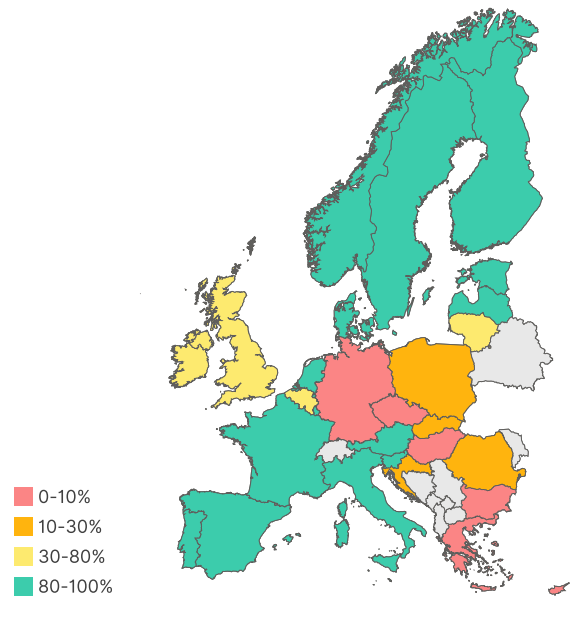
\includegraphics[width=0.75\linewidth]{figure/Smart_EU.PNG}
    \caption{Roll-out of smart meters among households \cite{ACER2024} }
    \label{fig:Smart_EU}
\end{figure}
     \end{center}
\end{column}
\begin{column}{0.50\textwidth}
\small	
 \boldrblue{20 EU countries out of 29} have regulated and non-regulated dynamic contract options for households \cite{ACER2024}
\hyperlink{ContractType}{\beamergotobutton{Table}},\hyperlink{USdata}{\beamergotobutton{US Data}},\hyperlink{options2}{\beamergotobutton{Details}},\hyperlink{UptakeContract2}{\beamergotobutton{Back }}
\hspace{2cm}
\end{column}
\end{columns}

\end{frame}


%%%%%%%%%%%%%%%%%%%%%%%%%%%%%%%%%%%%%%%%%%%%%%%%%%%%%%%%%%%%%%%%%%%%%%%%%%%%%%%%%%%%%%%%%%%%%%%%%%%%%%%%%%%%%%%%%%%%%%%%%%%%%%%%%%%%%%%%%%%%%%%%%%%%%%

\begin{frame}{Available technology and contract options}\label{options2}

% \begin{columns}

% \begin{column}{0.55\textwidth}  %%<--- here
%     \begin{center}
% \begin{figure}
%     \centering
%     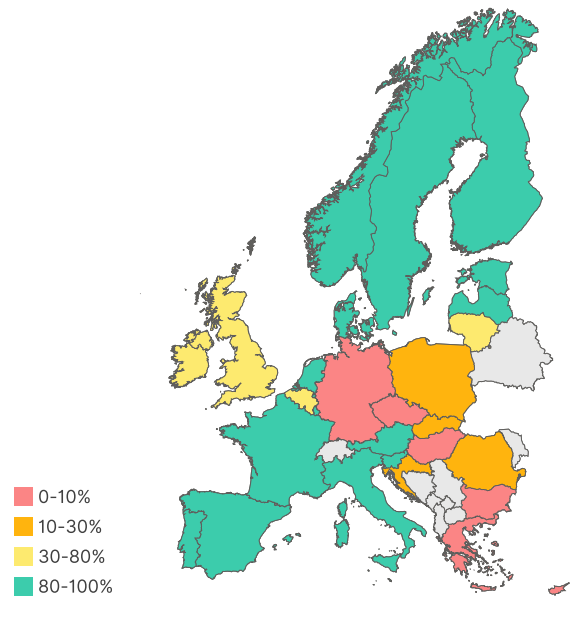
\includegraphics[width=0.75\linewidth]{figure/Smart_EU.PNG}
%     \caption{Roll-out of smart meters among households \cite{ACER2024} }
%     \label{fig:Smart_EU}
% \end{figure}
%      \end{center}
% \end{column}
% \begin{column}{0.50\textwidth}
% \small	
%  \boldrblue{20 EU countries out of 29} have regulated and non-regulated dynamic contract options for households \cite{ACER2024}

% \hspace{2cm}

\begin{figure}
    \centering
    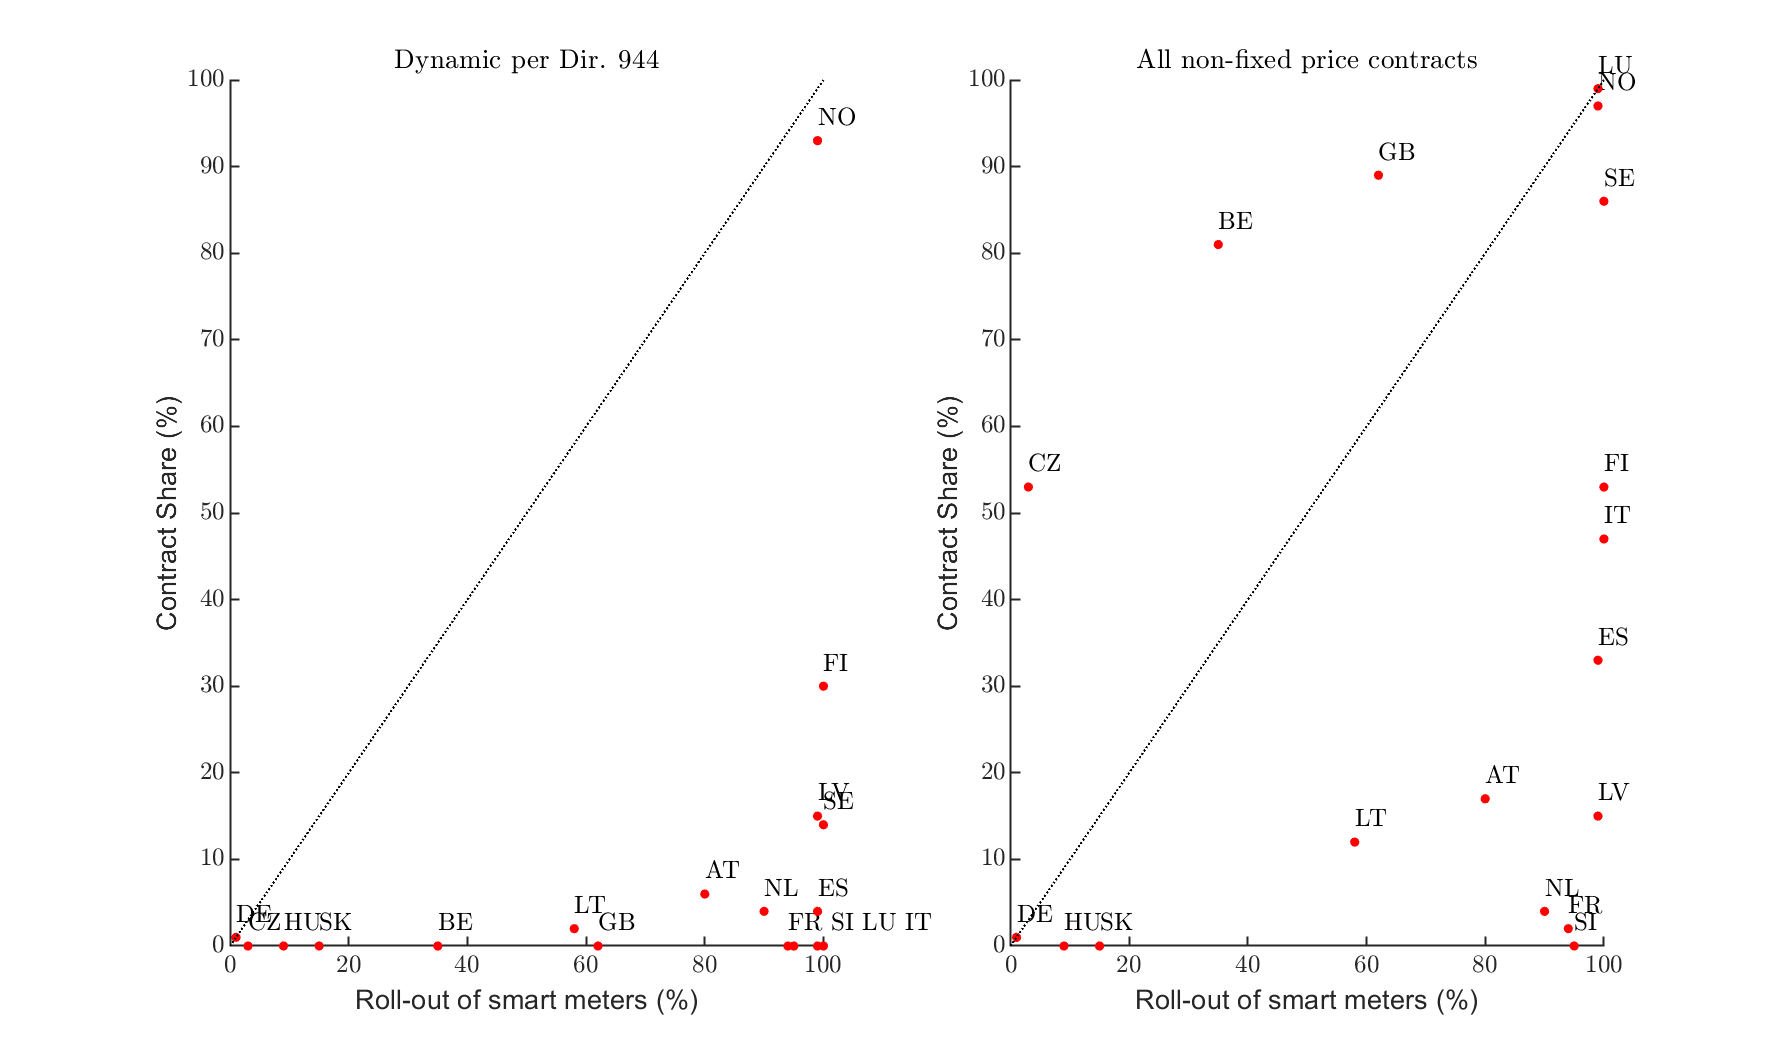
\includegraphics[width=1\linewidth]{figure/share_contract.PNG}
    \caption{Share of contract uptakes with respect to share of roll-out of smart meters among households (own calculation based on \cite{ACER2024}),\hyperlink{ContractType}{\beamergotobutton{Table}},\hyperlink{USdata}{\beamergotobutton{US Data}},\hyperlink{options1}{\beamergotobutton{Back}}}
    \label{fig:Smart_EU}
\end{figure}







% \end{column}
% \end{columns}



\end{frame}


%%%%%%%%%%%%%%%%%%%%%%%%%%
%%%%%%%%%%%%%%%%%%%%%%%%%%%%%%%%%%%%%%%%%%%%%%%%%%%%%%%%%%%%%%%%%%%%%%%%%%%%%%%%%%%%%%%%%%%%%%%%%%%%%%%%%%%%%%%%%%%%%%%%%%%%%%%%%%%%%%%%%%%%%%%%%%%%%%

\begin{frame}{Contract Options in the EU}\label{ContractType}

\begin{figure}
    \centering
    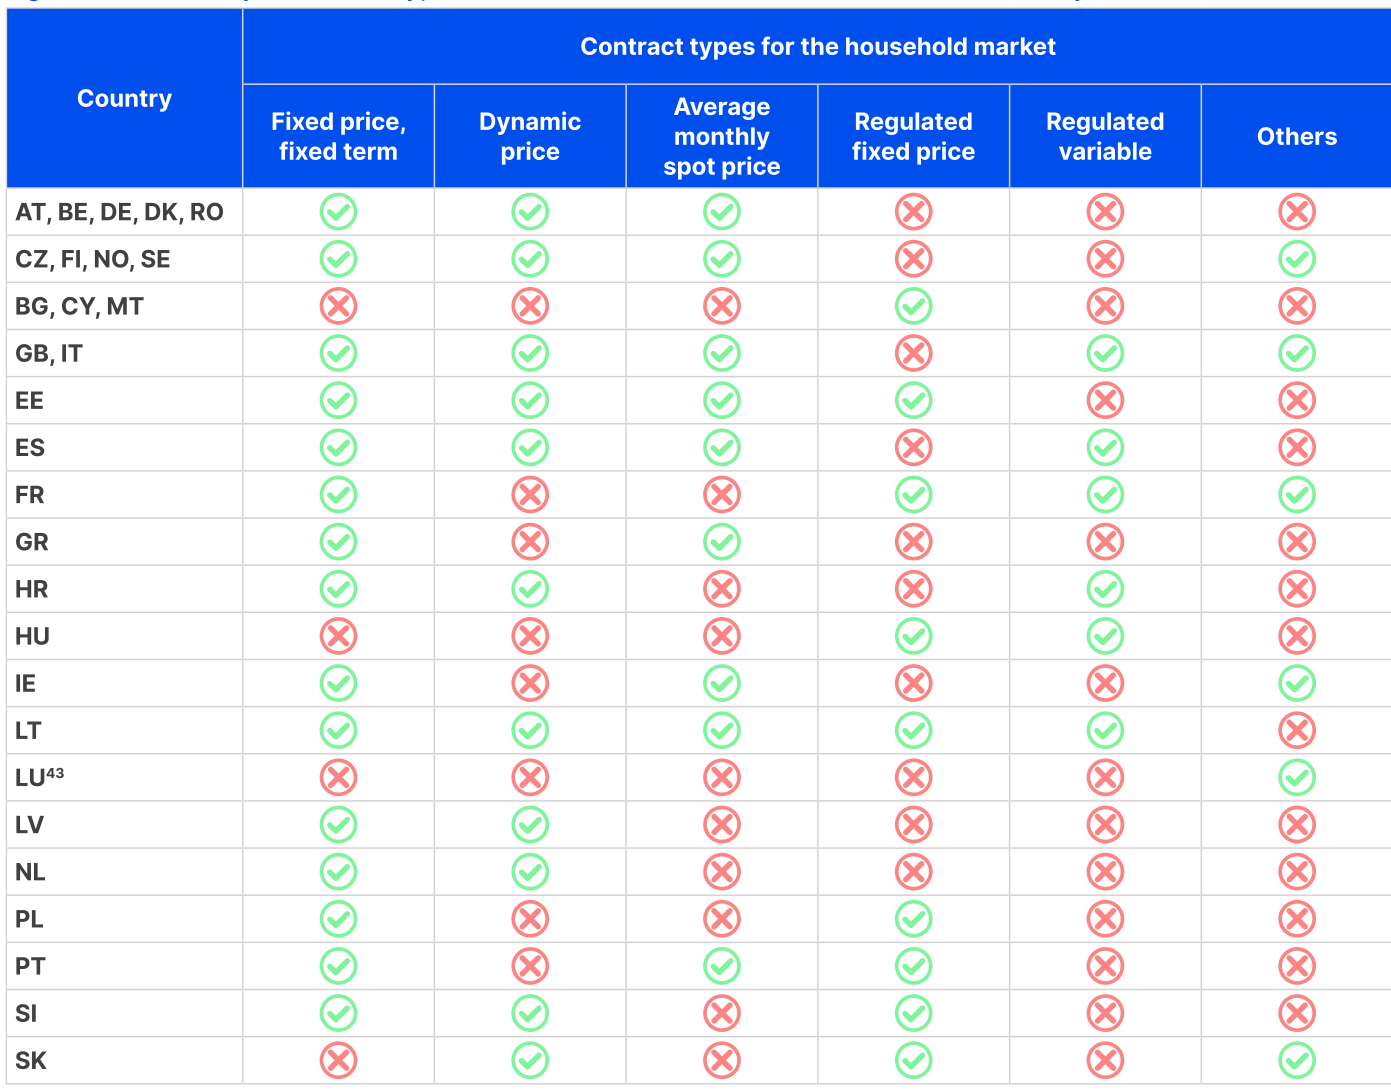
\includegraphics[width=0.8\linewidth]{figure/ContractType.PNG}
    \caption{Availability of different types of contracts to customers in the household electricity market in 2023 Country.\cite{ACER2024}  \hyperlink{options1}{\beamergotobutton{Back}} }
    \label{fig:ContractType}
\end{figure}
    
\end{frame}


%%%%%%%%%%%%%%%%%%%%%%%%%%%%%%%%%%%%%%%%%%%%%%%%%%%%%%%%%%%%%%%%%%%%%%%%%%%%%%%%%%%%%%%%%%%%%%%%%%%%%%%%%%%%%%%%%%%%%%%%%%%%%%%%%%%%%%%%%%%%%%%%%%%%%%

\begin{frame}{US Data}\label{USdata}

\begin{figure}
    \centering
    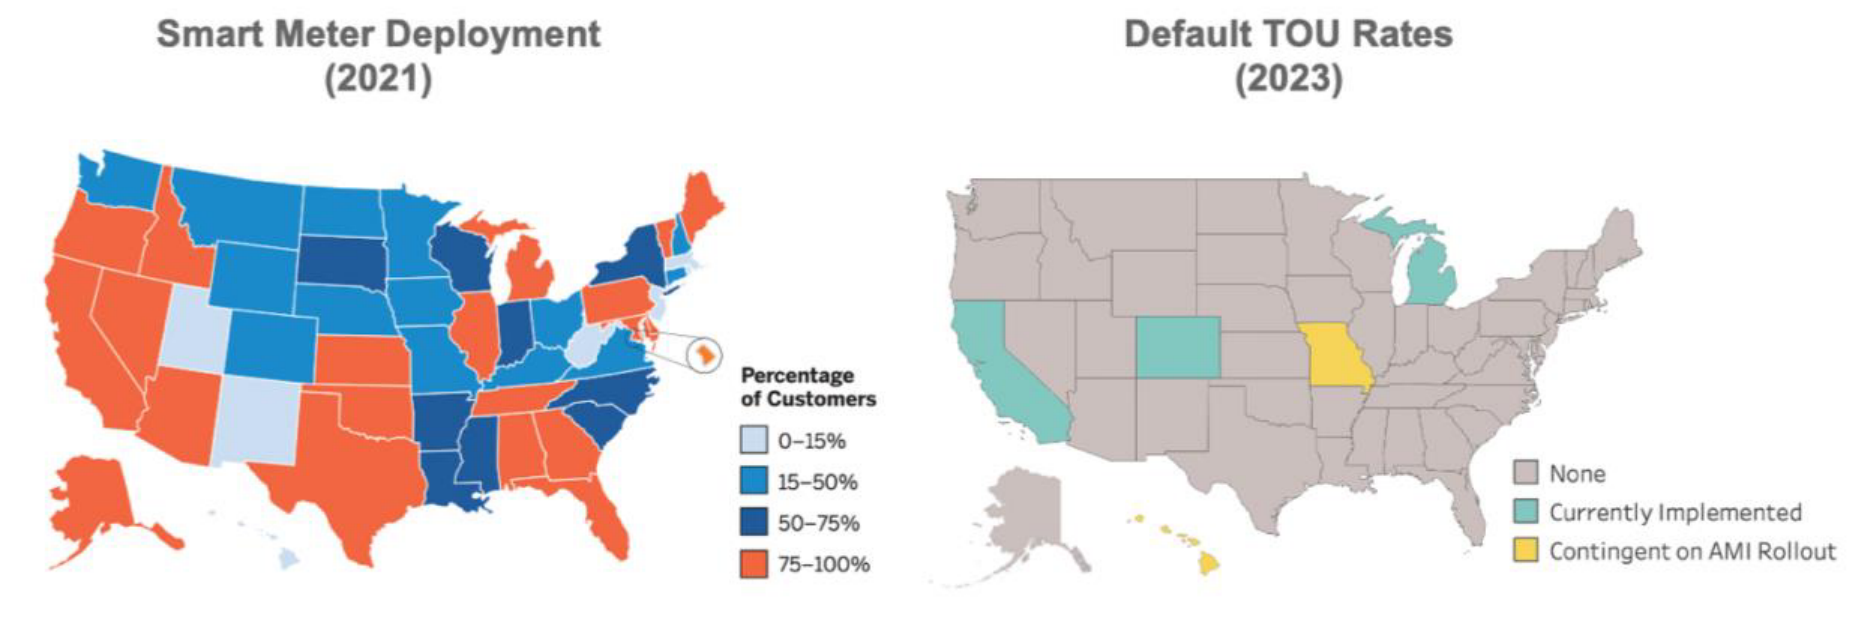
\includegraphics[width=1\linewidth]{figure/FP_Smart_US.PNG}
    \caption{Smart meter deployment among US households (left) and default TOU rate adoption (right). Default TOU rates are shown for each state's largest distribution utility. \cite{Turk2024}  \hyperlink{options1}{\beamergotobutton{Back}} }
    \label{fig:FP_Smart_US}
\end{figure}
    
\end{frame}

%%%%%%%%%%%%%%%%%%%%%%%%%%%%%%%%%%%%%%%%%%%%%%%%%%%%%%%%%%%%%%%%%%%%%%%%%%%%%%%%%%%%%%%%%%%%%%%%%%%%%%%%%%%%%%%%%%%%%%%%%%%%%%%%%%%%%%%%%%%%%%%%%%%%%%



\bibliography{bib}

\end{document}
